\section{Formalization}\label{sec:formal}
\liyi{This section might say too much, we might cut more here, and put more
  items in the compilation and implementation. }

\mz{                            %
  I am wondering if it's still a good idea to talk about syntax, semantics
  and types separately?
  %
  The key of the work is about tainted pointer, functions and blocks instead of
  the overview of the entire system.
  %
  Tearing those topics apart into 3 aspects can lead to incoherence.
  %
}

% \begin{itemize}
% \item Describe the types for checked-C as a graph. \dvh{I don't know what this means.}

% \item Describe the subtyping for checked-C types.
% \begin{itemize}
% \item State that the subtypes in Checked-C are transitive.
% \end{itemize}

% \item Describe the syntax of Checked-C

% \item Describe the semantics of Checked-C

% \item Describe the type system of Checked-C

% \item Describe the progress and preservation theorems, and outline the proofs.

% \item Describe the blame theorem and proof.

% \end{itemize}

% \ignore{
% \begin{figure}
%   \begin{center}
%     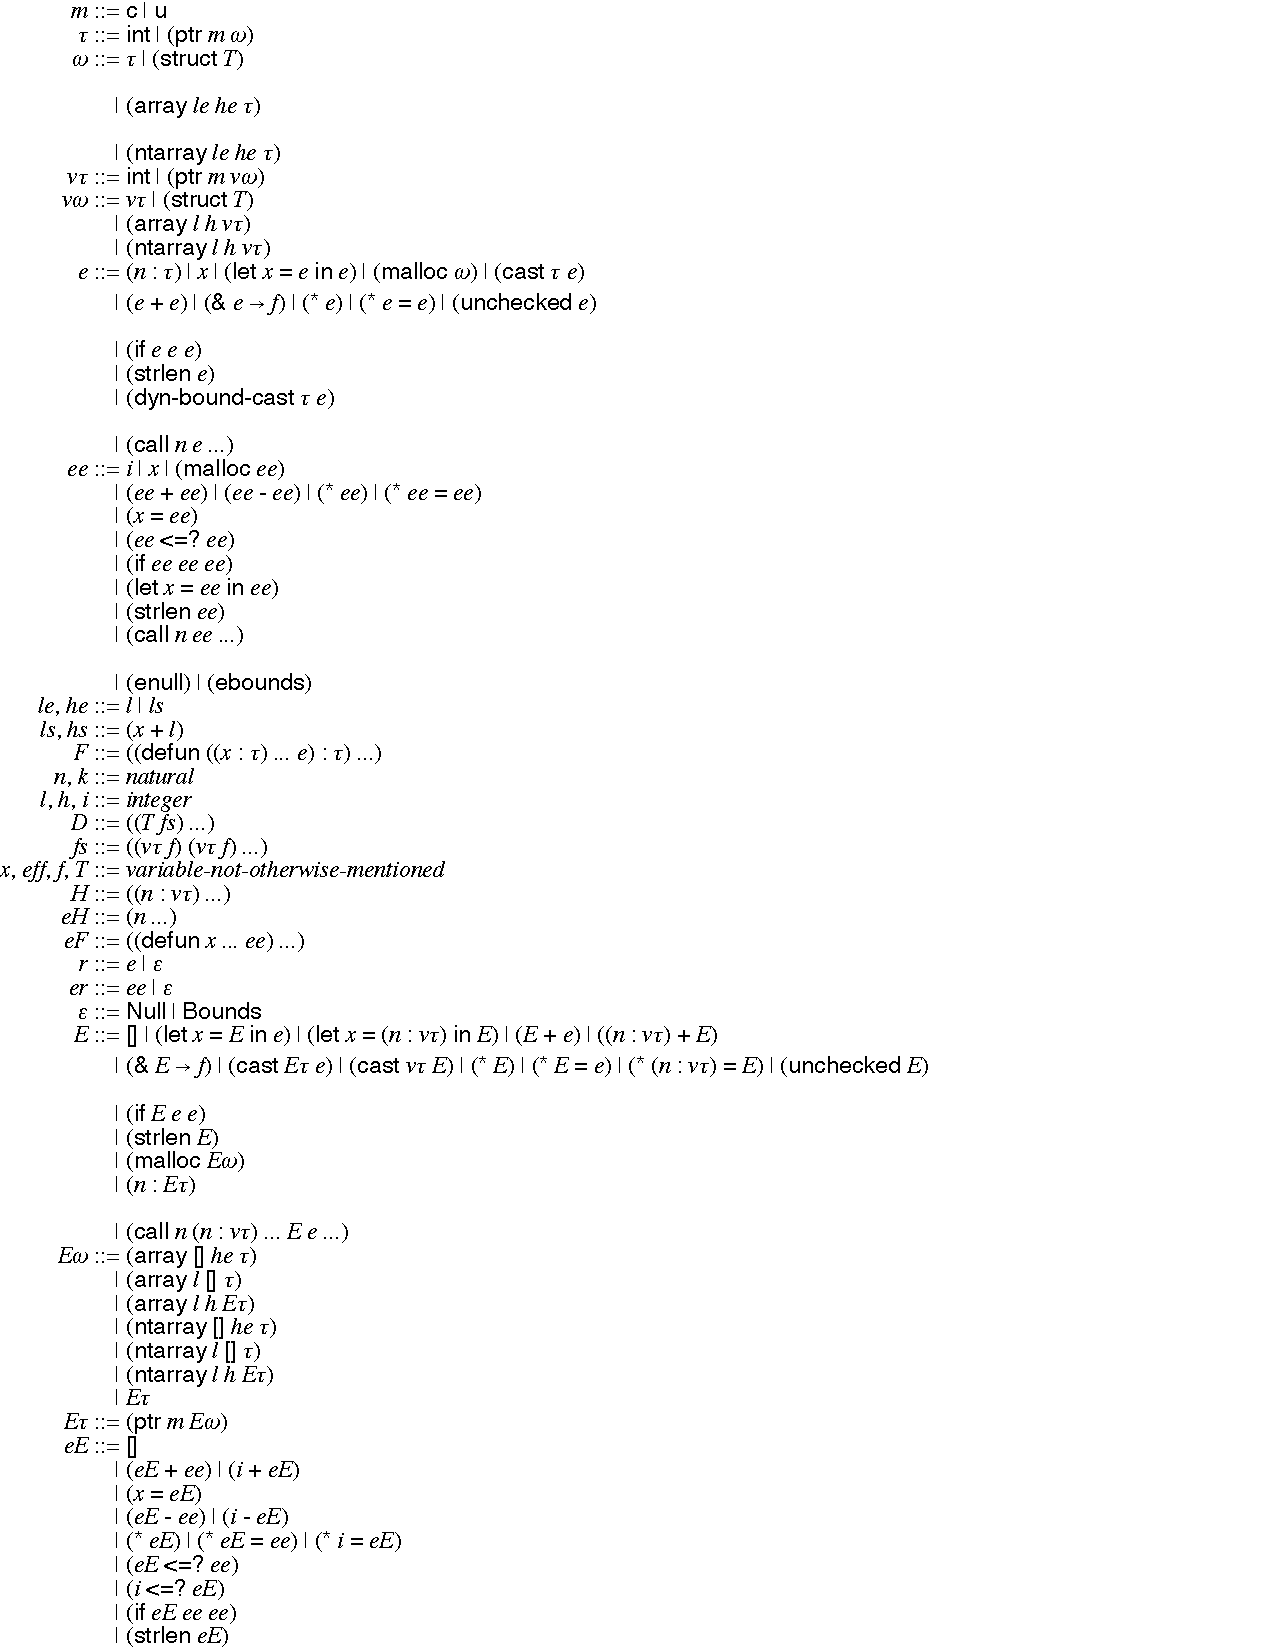
\includegraphics[height=6in]{syntax.pdf}
%   \end{center}
%   \caption{\lang: Syntax}
% \end{figure}

% \begin{figure}
%   \begin{center}
%     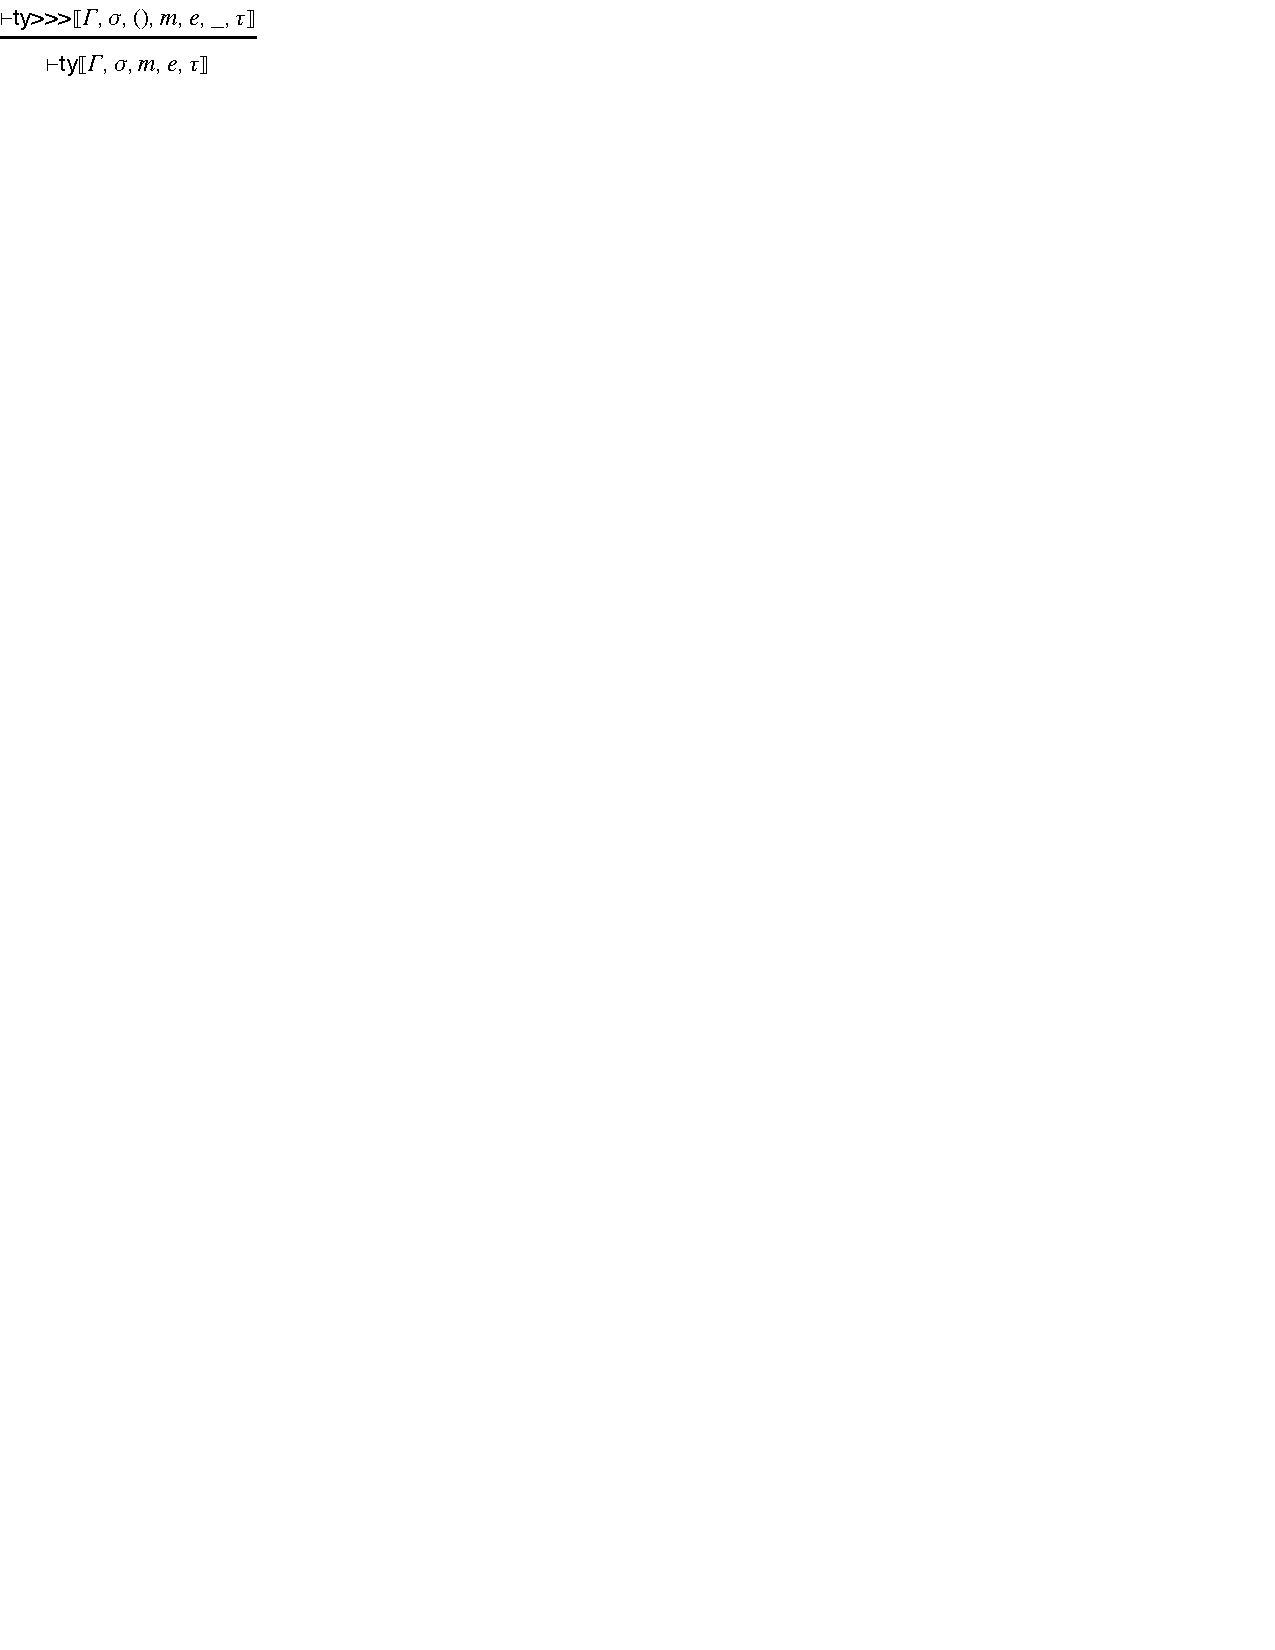
\includegraphics[height=6in]{types.pdf}
%   \end{center}
%   \caption{\lang: Typing}
% \end{figure}
% }
% \liyi{main text begins here. }

% \review{
% While reading the semantics, I found the fact that S-Def and S-DefNull are
%   applicable non-deterministically if n is 0 a bit confusing. Only when
%   reading the meta-theory section I realized that this is not a concrete issue
%   because well-formed heaps are such that $\mathcal{H}(0)$ is never defined. It
%   might be worth pointing this out early on. }
% \mwh{Done.}

\begin{figure}
  \small \centering
  \[ \hspace*{-1.2em}
\begin{array}{l}
\begin{array}{ll}
       \text{Variables:}~ x
& \text{Integers:}~n::=\mathbb{Z} 
\end{array}
\\[0.5em]

\begin{array}{llcllcl}

\text{Context Mode:} & m & ::= & \cmode \mid \umode \\[0.5em]

\text{Pointer Mode:} & \xi & ::= & m \mid \tmode \\[0.5em]

\text{Bound:} & b & ::= & n \mid x \plus n \\
              & \bvar & ::= & (b,b) \\[0.5em]
  
     \text{Word Type:}& \tau &::=& \tint\mid \tptr{\omega}{ \xi}
\\[0.5em]

\text{Type Flag:}&\kappa &::=& nt \mid \cdot
\\[0.5em]

\text{Type:}&\omega &::=& \tau \mid \tallarrayb{\bvar}{\tau} \mid \tfun{\overline{x}}{\overline{\tau}}{\tau}
\\[0.5em]

\text{Expression:}& e & ::= & 
\evalue{n}{\tau} \mid x \mid \ebinop{e}{e}\mid \ecast{\tau}{e} \mid \edyncast{\tau}{e}  \\[0.2em]
&&\mid& \estrlen{x} \mid\estar{e}\mid\eassign{e}{e}  \\[0.2em]
&&\mid& \elet{x}{e}{e} \mid \eif{e}{e}{e}
\\[0.2em]
&&\mid&  \emalloc{\xi}{\omega} \mid \ecall{e}{\overline{e}}
\\[0.2em]
&&\mid&\eunchecked{\overline{x}}{e}
\mid \echecked{\overline{x}}{e}

\end{array}
    \end{array}
  \]
  \caption{\lang Syntax}
  \label{fig:checkc-syn}
\end{figure}

\begin{figure}[t]
{\small
  \begin{mathpar}

  \inferrule[]
  {}
  {m \vdash \tint}

  \inferrule[]
  {\xi \wedge m\vdash \tau \\ \xi \le m}
  {m \vdash \tptr{\tallarrayb{\bvar}{\tau}}{\xi}}

  \inferrule[]
  {\xi \wedge m \vdash \tau\\ \xi \le m}
  {m \vdash \tptr{\tau}{\xi}}

  \inferrule[]
  {\xi \wedge m \vdash \tau\\ \xi \le m \\\\ \fv(\overline{\tau})\cup\fv(\tau)\subseteq \overline{x}}
  {m \vdash \tptr{(\tfun{\overline{x}}{\overline{\tau}}{\tau}}{\xi})}
  \end{mathpar}
}
{\footnotesize
\[
\begin{array}{l} 
\tmode \wedge \cmode = \umode \qquad \xi \wedge \umode = \umode
\qquad \cmode \wedge m = m 
\qquad  m_1 \wedge m_2 = m_2 \wedge m_1
\\[0.2em]
\xi \le \xi \qquad \tmode \le \xi
\end{array}
\\
\]
}
 \caption{Well-formedness for Types}
\label{fig:wftypes}
\end{figure}

%% \dvh{I don't understand the variable grammar.  What is $T$?  What is $\eta$?  I think $\cmode$ and $\umode$ should be in tt font.}
%% \liyi{T and $\eta$ can be moved to the appendix, they are useful only for struct types.}

% \review{
% - Furthermore, inspecting the code also suggests that the expression type (line 155) does not contain constructors for function calls (and I don't see a way to define functions either), conditionals, or strlen, and doesn't distinguish between the two forms of casting. All this contradicts figure 2, and should be clarified
% }
% \liyi{It is in the CheckedC.v file, 392. }
% \mwh{How is this answer helping the reviewer since you've added
%   nothing to the text? Maybe we should add something to an appendix
%   that matches the formalism shown in the paper to definitions in the
%   Coq file?}
% \liyi{The detailed explanation is in the appendix.}

This section describes the formal model of \systemname, named
\lang, making precise its syntax, semantics, and type system. It also
develops \lang's meta-theory, including the type soundness, non-exposure, and non-crashing
theorems.

\subsection{Syntax}\label{sec:syntax}

The syntax of \lang is given by the expression-based
language presented in Fig.~\ref{fig:checkc-syn}.
\liyi{why can we just say in.. }

There are two type notions in \lang.  Types $\tau$ classify
word-sized values including integers and pointers, while types
$\omega$ classify multi-word values such as arrays, null-terminated
arrays, functions, and single-word-size values. \liyi{Is this a good way? the differences are mainly for the result types vs type elements. }
%
Pointer types ($\tptr{\omega}{\xi}$) include a pointer mode annotation 
($\xi$, the difference between context and pointer modes is introduced shortly below)
that is either checked (\cmode), tainted (\tmode), or unchecked (\umode),
and a type ($\omega$) denoting valid values that can be pointed to.
\liyi{a little too much? Should we assume people know what pointer type is?}
\liyi{never mention $m$. }
Array types include both the type of
elements ($\tau$) and a bound ($\bvar$) comprised of an upper and
lower bound on the size of the array ($(b_l,b_h)$). Bounds $b$ are
limited to integer literals $n$ and expressions $x + n$.
Whether an array pointer is null terminated or not is determined by annotation
$\kappa$, which is $nt$ for null-terminated arrays, and $\cdot$
otherwise (we elide $\cdot$ when writing types).
\liyi{should have a better way. }
% 

\mz{Let's zero in on the function pointer and the mode context formalism.
We can say something like ``bounds and array ptrs have been studied in [...]''
already.
}

% 
\lang{} function types ($\tfun{\overline{x}}{\overline{\tau}}{\tau}$)
reflect its dependent function declarations,
where $\overline{x}$ represents
a list of \tint{} type variables in a dependent function header
that bind bound variables appearing in $\overline{\tau}$ and $\tau$.
\liyi{need to fix, do not understand. }
We have a well-formed requirement for a function type;
that is, all variables in $\overline{\tau}$ and $\tau$ are bounded by $\overline{x}$.
Here is the
corresponding \systemname syntax for these types:
\[\hspace*{-0.5em}
\begin{array}{l}
\begin{array}{rcl}
$\code{array_tptr<}$\tau$\code{> : count(}$n$\code{)}$
&\Leftrightarrow& \tarrayptr{0}{n}{\tau}{\tmode}
\\[0.2em]
$\code{nt_array_ptr<}$\tau$\code{> : count(}$n$\code{)}$
&\Leftrightarrow& \tntarrayptr{0}{n}{\tau}{\cmode}
\end{array}
\\[0.2em]
$\code{tptr<(int)(nt_array_tptr<}$\tau$\code{> : count(}$n$\code{),}$\\
\qquad\qquad$\code{nt_array_tptr<}$\tau$\code{>)>: count(}$n$\code{))>}$
\\[0.2em]
\Leftrightarrow\;\; $\tptr{(\tfun{n}{ \tntarrayptr{0}{n}{\tau}{\tmode} \times \tntarrayptr{0}{n}{\tau}{\tmode}}{\tint})}{\tmode}$
\end{array}
\]
As a convention we write $\tptr{\tarrayb{b}{\tau}}{\cmode}$ to mean
$\tptr{\tarray{0}{b}{\tau}}{\cmode}$, so the firs two examples above could
be rewritten $\tptr{\tarrayb{n}{\tau}}{\cmode}$ and
$\tptr{\tntarrayb{n}{\tau}}{\cmode}$, respectively.
\liyi{we might just cut nt-array ptrs. it seems to me that nt-array ptrs are not important. }

\lang expressions include literals ($n\!:\!\tau$), variables ($x$),
 addition ($\ebinop{e_1}{e_2}$), static casts ($\ecast{\tau}{e}$), 
dynamic casts ($\edyncast{\tau}{e}$) \footnote{assumed at compile-time and verified at run-time, see \Cref{app:main}},
the \texttt{strlen} operation ($\estrlen{x}$),
pointer dereference and assignment ($\estar{e}$)
and ($\eassign{e_1}{e_2}$), resp.),
let binding ($\elet{x}{e_1}{e_2}$),
conditionals ($\eif{e}{e_1}{e_2}$),
memory allocation ($\emalloc{\xi}{\omega}$), 
function calls ($\ecall{e}{\overline{e}}$),
unchecked blocks ($\eunchecked{\overline{x}}{e}$), and checked blocks ($\echecked{\overline{x}}{e}$).
% \review{III.A.: the "dynamic cast" terminology may be briefly confused for C++'s
%   RTTI-based dynamic cast feature}
% \mwh{Added reference back to Section 2-B}

Integer literals $n$ are annotated with a type $\tau$ which can be either
$\tint$, or $\tptr{\omega}{\xi}$ in the case $n$ is being used as 
a heap address (this is useful for the semantics);
$\evalue{0}{\tptr{\omega}{\xi}}$ (for any $\xi$ and $\omega$) represents the $\enull$ pointer, as usual. 
The $\texttt{strlen}$ expression operates on variables $x$
rather than arbitrary expressions to simplify managing
bounds information in the type system; the more general case can be
encoded with a \code{let}. We use a less verbose syntax for dynamic bounds
casts; e.g., the following %

\code{dyn_bounds_cast<array_ptr<}$\tau$\code{>>(}$e$\code{, count(}$n$\code{))}

\noindent
becomes $\edyncast{\tptr{\tarrayb{n}{\tau}}{\cmode}}{e}$. 

\mz{
  I would say that let's just focus on uncheckd and checked.
  %
  We can make an simple example that contains a function pointer with dependent
  parameters; then, explain in great detail what that means.
  % 
  Instead of rephrasing the meaning of symbols, we might as well direct the reader
  to the appendix/previous work for tech details on the last paper. 
}

\liyi{should we bring out the difference? since readers might not even know the previous paper.}
Compared to the former \checkedc model \cite{li22checkedc},
there are four differences.
First, the \systemname type annotations have well-formed restrictions in \Cref{fig:wftypes}, 
for maintaining non-exposure.
Mainly, in a nested pointer $\tptr{(... \tptr{\tau}{\xi_2} ...)}{\xi_1}$, $\xi_2\le \xi_1$.
It is worth noting that pointer modes are a three point partial order ($\le$),
where $\tmode$ is the infimum, and
$\xi\wedge m$ is a special meet operation that projects pointer modes onto context modes,
such that $\tmode$ is projected as $\umode$.
\liyi{not clear. }
Second, $\emalloc{\xi}{\omega}$ includes a mode flag
$\xi$ for allocating different pointers in different heaps.
We disallow $\omega$ to be a function type ($\tfun{\overline{x}}{\overline{\tau}}{\tau}$).
Third, the first expression $e$ in a function call ($\ecall{e}{\overline{e}}$) represents a function pointer.
\liyi{might need to bring out what is the difference of previous ones.}
Fourth, $\echeckedtext$ blocks are added to the system, 
which permits the nested context-switching between $\echeckedtext$ (represented by context mode $\cmode$)
and $\euncheckedtext$ (represented by context mode $\umode$) code regions.
One example usage of the nested context-switching is the checked function callbacks inside 
an unsafe region in \Cref{fig:checkedc-example-2} and \ref{fig:checkedc-example-3}.
To guarantee the non-exposure safety,
 we extend the $\echeckedtext$ and $\euncheckedtext$ block syntax to be 
$\echecked{\overline{x}}{e}$ and $\eunchecked{\overline{x}}{e}$:
$\overline{x}$ restricts all free variables appearing in $e$, and they cannot be checked pointers.

\lang aims to be simple enough to work with, but powerful enough to
encode realistic \systemname idioms. For example, mutable local
variables can be encoded as immutable locals that point to the heap;
the use of \code{&} can be simulated with \code{malloc};
and loops can be encoded as recursive function calls. \code{struct}s are
not in Fig.~\ref{fig:checkc-syn} for space reasons, but they are
actually in our model, and developed in
\iftr
Appendix~\ref{appx:struct}.
\else
the supplemental report~\cite{checkedc-tech-report}.
\fi
C-style \code{union}s have no safe typing
in \checkedc, so we omit them.
\liyi{last sentence can be cut. }


% \mwh{NOTE: COULD WORK THE FOLLOWING INTO THE ABOVE DESCRIPTION OF
%   POINTERS: Array and NT-array types have two relative bounds, whose structures
% can be either an integer or a variable plus an integer. For example,
% if we have the expression
% $x\texttt{=}\emalloc{\tarrayb{(0,10)}{\tint}}$, $x$ then has the type
% $\tptr{\tarrayb{10}{\tint}}{\cmode}$, which represents an array
% pointer of size $10$. The bounds ($(b_l,b_h)$ in
% $\evalue{p}{\tptr{\tarrayb{(b_l,b_h)}{\tau}}{m}}$) indicate relative
% offsets from this pointer of the accessible memory, i.e., $p+b_l$ and
% $p+b_h$. As such, a pointer can only be directly dereferenced if 0 is
% included within the annotated range.  If following the $\emalloctext$
% operation, we execute $*(x-1)$ and $*(x\plus 10)$. The two expressions
% are not valid, because the type of the two expressions $(x-1)$ and
% $(x\plus 10)$ are $\tarrayptr{1}{11}{\tint}{\cmode}$ and
% $\tarrayptr{-10}{0}{\tint}{\cmode}$ and $0$ in these two cases are not
% in the ranges: $[1,11)$ and $[-10,0)$. Thus, in order for a $\cmode$
% pointer with type $\tarrayptr{b_l}{b_h}{\tint}{\cmode}$ to be
% accessible in \checkedc, $0$ must be in the range of $[b_l,b_h)$.}

\begin{figure}
{\small
$\hspace*{-1.2em}
    \begin{array}{l}
    \begin{array}{lll}
e & ::= & \ldots \mid \ret{x}{\evalue{n}{\tau}}{e}\\
r & ::= & e \mid \enull \mid \ebounds\\
E &::=& \Box \mid \ebinop{E}{e} \mid \ebinop{\evalue{n}{\tau}}{E}\mid \ecast{\tau}{E} \mid \edyncast{\tau}{E} \mid\estar{E}\mid\eassign{E}{e}\\[0.2em]
&&\mid\eassign{\evalue{n}{\tau}}{E}\mid \elet{x}{E}{e}\mid \eif{E}{e}{e}\\[0.2em]
&&\mid \ecall{E}{\overline{e}} \mid \ecall{\evalue{n}{\tau}}{\overline{E}} \mid 
\eunchecked{\overline{x}}{E}
\mid \echecked{\overline{x}}{E}


\end{array}
\\ \\
    \end{array} 
$
  \begin{mathpar}
    \inferrule{ m=\mode(E) \\
      e=E[e'] \\
      (\varphi,\heap,e') \longrightarrow (\varphi',\heap',e'')}
    {(\varphi,\heap,e)\longrightarrow_{m} (\varphi',\heap',E[e''])}

    \inferrule{ \umode=\mode(E) \\
      e=E[e'] \\
      \tau=\type(e')}
    {(\varphi,\heap,e)\longrightarrow_{\umode} (\varphi,\heap,E[\evalue{0}{\tau}])}

  \end{mathpar}
}
{\footnotesize
\[
\begin{array}{l} 
\mode(E)=\mode'(E,\cmode)
\\[0.2em]
\mode'(\Box,m)=m
\\[0.2em]
\mode'(\eunchecked{\overline{x}}{E},m)=\mode'(E,\umode)
\\[0.2em]
\mode'(\echecked{\overline{x}}{E},m)=\mode'(E,\cmode)
\\[0.2em]
\mode'(\alpha({E}),m)=\mode'(E,m)\;\;{[\emph{owise}]}
\end{array}
\\
\]
}
  \caption{\lang Semantics: Evaluation}
  \label{fig:c-context}
\end{figure}

\subsection{Semantics}\label{sec:semantics}

% The semantics
% gives an independent account of spatial safety in \lang by
% checking pointer bounds based on the annotations carried on types at
% run-time.  While this account makes clear that bounds checking occurs
% as expected, it suggests an implementation that uses fat pointers to
% carry bounds.  We resolve this tension in the subsequent section on
% compilation and show that an implementation faithful to the semantics
% can be obtained without fat pointers.  
% \review{repeat that the stack is immutable at this point?}
% \liyi{Is it? Is the stack immutable? What does the immutable mean? 
%   In a stack, the variable values can be changed? Right?
%   The pointer address itself cannot be changed once it is created, but the stack variable content can be updated?  }
% \mwh{It certainly seems to be immutable: Your create stack frames
%   using let binding, and the let-bound variables will always be bound
%   to the same things. I.e., stack cells are immutable.}

% \review{this raises a fair amount of questions regarding the treatment of the
%   NULL pointer at this stage of the paper... is it modeled as 0, as returned by
%   `malloc`? are dynamic checks inserted by CheckedC to guarantee that no NULL
%   pointer is dereferenced?}
% \mwh{Yes, it is modeled as 0, and the semantics checks for
%   dereferences of 0. }

The operational semantics for \lang is defined as a small-step
transition relation with the judgment $ (\varphi,\heap,e)
\longrightarrow_m (\varphi',\heap',r)$.
\liyi{do we need to say judgment here? }
 Here, $\varphi$ is a
\emph{stack} mapping from variables to values $\evalue{n}{\tau}$ and
$\heap$ is a \emph{heap} that is partitioned into two parts ($\cmode$ and $\umode$ heaps), each of which
maps addresses (integer literals) to values $\evalue{n}{\tau}$.
A $\cmode$ pointer is mapped to a heap location in the $\cmode$ heap, 
while a $\tmode$ and $\umode$ pointer represents a $\umode$ heap location.
We wrote $\heap(m,n)$ to retrieve the $n$-location heap value in the $m$ heap,
and $\heapup{m}{n}{\evalue{n'}{\tau}}$ 
to update location $n$ with the value $\evalue{n'}{\tau}$ in the $m$ heap.
It is worth noting that \systemname is not a fat-pointer system;
thus, in every heap update, the value type annotation remains the same through program executions.
Additionally, for both stack and heap, 
we ensure $\fv(\tau)=\emptyset$ for all the value type annotations $\tau$.

While heap bindings can change, stack bindings are immutable---once
variable $x$ is bound to $\evalue{n}{\tau}$ in $\varphi$, that binding will not
be updated. 
We can model mutable stack variables as pointers into the
mutable heap.
\liyi{why we need this sentence? }
As mentioned, value $\evalue{0}{\tau}$
represents a $\enull$ pointer when $\tau$ is a pointer type.
Correspondingly, $\heap(m,0)$ should always be undefined.
The relation steps to a \emph{result} $r$,
which is either an expression or a $\enull$ or $\ebounds$ failure,
represent a null-pointer dereference or out-of-bounds access,
respectively. Such failures are a \emph{good} outcome; stuck states
(non-value expressions that cannot transition to a result $r$)
characterizing undefined behavior.
%
The context mode $m$ (in $\longrightarrow_{m}$) indicates whether the
stepped redex within $e$ was in a checked ($\cmode$) or
unchecked ($\umode$) region.

The rules for the main operational semantics
judgment---\emph{evaluation}---are given at the middle of
Fig.~\ref{fig:c-context}.
The first rule takes an expression $e$, decomposes
it into an \emph{evaluation context} $E$ and a sub-expression $e'$
(such that replacing the hole $\Box$ in $E$ with $e'$ would yield
$e$), and then evaluates $e'$ according to the \emph{computation}
  relation $(\varphi,\heap,e') \longrightarrow (\varphi,\heap,e'')$,
whose rules are given in Fig.~\ref{fig:semantics}, discussed
shortly. 
The second rule describes the exception handling 
for possible crashing behaviors in unchecked regions.
A $\umode$ mode operation can non-deterministically crash
and the \systemname sandbox mechanism recovers
the program to a safe point ($\evalue{0}{\tau}$)
and continues with the existing program state.
\liyi{is non-deterministically crashed or non-determinstically transitioned to some place. }
Evaluation contexts $E$ define a standard left-to-right evaluation order. (We explain the
$\ret{x}{\mu}{e}$ syntax shortly.)
There are other rules for describing the halts of evaluation to $\enull$ and $\ebounds$ states in \Cref{app:main}.
\liyi{might not need this. }

%\footnote{This approach is that of the PLT Redex model of \lang; the Coq
%development uses a slightly simpler syntax to achieve the same
%effect.}
% \review{the special case raises questions, e.g. why is this syntax-driven and
%   not type-driven? }
% \liyi{This describes the semantic transition rules. We are using context evaluation framework to define the transition rules as the $E$ definition in Fig.3. like $\frac{x \Rightarrow y}{x+z \Rightarrow y + z}$, I don't know how type-driven can help us define translation rules.  }
% \mwh{Don't follow the above. I don't see this ``context transition
%   rule'' anywhere, and I'm not sure how it would fire, if we had it.}
% \liyi{The comment seems to confuse the meaning of the text about the if-then-else rules. Making the rule specific will help. }
The $\mode$ function  at the bottom of Fig.~\ref{fig:c-context}
describes the context mode determination in each evaluation step based on the context $E$.
\liyi{understood? }
For any program execution, the function starts the mode computation with $\cmode$ ($\mode(E)=\mode'(E,\cmode)$).
The result context mode depends on where $\Box$ locates.
If it occurs within $E$ in $(\eunchecked{\overline{x}}{E})$
that has no surrounding $\echeckedtext$ block,
the mode is $\umode$; otherwise, the mode is $\cmode$.
$\mode'(\alpha({E}),m)=\mode'(E,m)$ represent other construct cases 
that are not $\echeckedtext$ and $\euncheckedtext$; in such case, 
the function recursively traverses the sub-context to find the context mode.
\liyi{may be too low-level detailed. describe it in a high level. }

\mz{
  I don't see the thesis of these first a few paragraphs. 
  %
  And, what's the motivation of mode? How on earth this setup solves the
  problem?
  %
  If we're explaining reduction in context, shall we delay the introduction of
  this context mode now?
}

% For a term $e$, $C$ is a context if any
% only if it contains a $\Box$ hole term in one of the subterm position
% in $e$. $\Box$ indicates the break point where we split $e$ into $C$
% and a subterm $e'$ such that $C[e'] = e$.  For a function call
% $\ecall{f}{\overline{e}}$, a valid context ($\overline{C}$) is defined
% as any one of the elements in the list $\overline{e}$ being a
% context. We show a rule of the upper level \checkedc semantics. The
% rule splits a term $e$ into a context $C$ and redex $e'$.  If subterm
% $e'$ is transitioned to $e_a$, $C[e']$ is transitioned to
% $C[e_a]$.

\begin{DIFnomarkup}
\begin{figure*}[t]
{\small
  \begin{mathpar}
        \inferrule[S-DefC]{\heap(\cmode,n)=\evalue{n_a}{\tau_a} }
    {(\varphi,\heap,\estar{\evalue{n}{\tptr{\tau}{c}}}) \longrightarrow (\varphi,\heap,\evalue{n_a}{\tau})}

    \inferrule[S-AssignArrC]{\heap(\cmode,n)=\evalue{n_a}{\tau_a}\\ 0 \in [n_l,n_h) }
      {(\varphi,\heap,\eassign{\evalue{n}{\tallarrayptr{n_l}{n_h}{\tau}{\cmode}}}{\evalue{n_1}{\tau_1}}) \longrightarrow (\varphi,\heapup{\cmode}{n}{\evalue{n_1}{\tau_a}},\evalue{n_1}{\tau})}

        \inferrule[S-DefT]{\heap(\umode,n)=\evalue{n_a}{\tau_a}
         \\  \emptyset;\heap ; \emptyset \vdash_{\umode}\evalue{n_a}{\tau} }
    {(\varphi,\heap,\estar{\evalue{n}{\tptr{\tau}{\tmode}}}) \longrightarrow (\varphi,\heap,\evalue{n_a}{\tau})}

    \inferrule[S-AssignArrT]{\heap(\umode,n)=\evalue{n_a}{\tau_a}\\ 0 \in [n_l,n_h)
               \\  \emptyset;\heap ; \emptyset \vdash_{\umode}\evalue{n_1}{\tau} }
      {(\varphi,\heap,\eassign{\evalue{n}{\tallarrayptr{n_l}{n_h}{\tau}{\tmode}}}{\evalue{n_1}{\tau_1}}) \longrightarrow (\varphi,\heapup{\umode}{n}{\evalue{n_1}{\tau_a}},\evalue{n_1}{\tau})}

    \inferrule[S-DefNull]{}{(\varphi,\heap,\estar{\evalue{0}{\tptr{\omega}{\cmode}}}) \longrightarrow (\varphi,\heap,\enull)}

    \inferrule[S-Cast]
              {}
              {(\varphi,\heap,\ecast{\tau}{\evalue{n}{\tau'}}) \longrightarrow (\varphi,\heap,\evalue{n}{\varphi(\tau)})}

    \inferrule[S-RetEnd]{}{(\varphi,\heap,\ret{x}{\evalue{n}{\tau}}{\evalue{n'}{\tau'}}) \longrightarrow (\varphi,\heap,\evalue{n'}{\tau'})}

        \inferrule[S-Let]{}{(\varphi,\heap,\elet{x}{\evalue{n}{\tau}}{e}) \longrightarrow (\varphi,\heap,\ret{x}{\evalue{n}{\tau}}{e})}

    \inferrule[S-RetCon]{ (\varphi[x\mapsto \evalue{n}{\tau}],\heap,e) \longrightarrow (\varphi',\heap',e')}{(\varphi,\heap,\ret{x}{\evalue{n}{\tau}}{e}) \longrightarrow (\varphi'[x\mapsto \varphi(x)],\heap',\ret{x}{\varphi'(x)}{e'})}

    \inferrule[S-Unchecked]{}{(\varphi,\heap,\eunchecked{\overline{x}}{\evalue{n}{\tau}}) \longrightarrow (\varphi,\heap,\evalue{n}{\tau})}

    \inferrule[S-FunC]{ \Xi(\cmode,n) = \tau\;(\evalue{\overline{x}}{\overline{\tau}})\;(\cmode,e)}
        {(\varphi,\heap,\ecall{\evalue{n}{(\tptr{\tau}{\cmode})}}{{\evalue{\overline{n_a}}{\overline{\tau_a}}}}) \longrightarrow
   (\varphi,\heap, \mathtt{let}\;\overline{x}={\evalue{\overline{n}}{(\overline{\tau}[\overline{n} / \overline{x}])}}\;\mathtt{in}\;\ecast{\tau[\overline{n} / \overline{x}]}{e})}

    \inferrule[S-Checked]{}{(\varphi,\heap,\echecked{\overline{x}}{\evalue{n}{\tau}}) \longrightarrow (\varphi,\heap,\evalue{n}{\tau})}

    \inferrule[S-FunT]{ \Xi(\umode,n) = \tau\;(\evalue{\overline{x}}{\overline{\tau}})\;(\tmode,e)
                  \\ \emptyset;\heap ; \emptyset \vdash_{\umode}\evalue{n}{\tptr{\tau}{\tmode}}}
        {(\varphi,\heap,\ecall{\evalue{n}{(\tptr{\tau}{\tmode})}}{{\evalue{\overline{n_a}}{\overline{\tau_a}}}}) \longrightarrow
   (\varphi,\heap, \mathtt{let}\;\overline{x}={\evalue{\overline{n}}{(\overline{\tau}[\overline{n} / \overline{x}])}}\;\mathtt{in}\;\ecast{\tau[\overline{n} / \overline{x}]}{e})}


 % \inferrule[S-IfNTNot]{\varphi(x)=\evalue{n}{\tntarrayptr{n_l}{n_h}{\tau}{\cmode}} \\ \heap(n)\neq 0\\ 0 < n_h}
 %            {(\varphi,\heap,\eif{\estar{x}}{e_1}{e_2}) \longrightarrow (\varphi,\heap,e_1)}

\end{mathpar}
}
% {\footnotesize
% \begin{center}
% $
% \begin{array}{l}
% \tau[\overline{n} / \overline{x}]\texttt{(with types }\evalue{\overline{x}}{\overline{\tau}}\texttt{)}\triangleq \forall n_i\in\overline{n}\;x_i\in\overline{x}\;\tau_i\in\overline{\tau}\;.\;\tau_i = \tint \Rightarrow \tau[n_i / x_i]\\[0.2em]
% \mathtt{let}\;\overline{x}=\overline{e}\;\mathtt{in}...\triangleq \mathtt{let}\;x_0=e_0\;\mathtt{in}\;\mathtt{let}\;x_1=e_1\;\mathtt{in}...
% \end{array}
% $
% \end{center}
% }
\caption{\lang Semantics: Computation (Selected Rules)}
\label{fig:semantics}
\end{figure*}
\end{DIFnomarkup}

\begin{figure}[t]
{\small
{\captionsetup[lstlisting]{margin = 8 mm}
  \begin{lstlisting}[xleftmargin=8 mm]
nt_array_ptr<char> safe_strcat
   (nt_array_ptr<char> dst : count(n),
    nt_array_ptr<char> src : count(0), int n) {
  int x = strlen(dst);
  int y = strlen(src);
  nt_array_ptr<char> c : count(n) =
    dyn_bounds_cast
           <nt_array_ptr<char>>(dst,count(n));
    // sets c == dst with bound n (not x)
  if (x+y < n) {
    for (int i = 0; i < y; ++i)
      *(c+x+i) = *(src+i);
    *(c+x+y) = '\0';
    return dst;
  }
  return null;
}
  \end{lstlisting}
}
}
\caption{Implementation of safe \code{strcat}}
\label{fig:strcat-ex}
\end{figure}

% \review{Fig4: it was hard to tell which cases were stuck states, or could reduce
%   owing to a rule that was not shown}
% \mwh{Stuck states are those where the expression is a non-value and
%   not $\enull$ or $\ebounds$. Updated III-B and III-D.}
% \review{Fig4: can the rules be presented in the same order they were introduced in
%   the paper?}
% \liyi{ Reordered }

% \review{Fig4: S-FUN: $\vec\tau_a$ seems unused; why?}
% \liyi{the list of $\tau_a$ is a list of input argument types. These
%   are used during type checking, but not during evaluation (as is
%   typical).} 

% LEO: This has an overfull line...?

Fig.~\ref{fig:semantics} shows selected rules for the computation relation.

\ignore{
 in
Fig.~\ref{fig:strcat-ex},
  which defines a 
  safe version of \code{strcat} (using actual Checked C syntax).  The
  function takes a target 
  pointer \code{dst} of capacity \code{n}, where the first null
  character (determined by \code{strlen}) is at index \code{x} where
  $0 \leq $\code{x}$ \leq n$. It concatenates the \code{src} buffer to
  the end of \code{dst} as long as \code{dst} has sufficient space.}

% Below, we introduce low-level transition semantics for some case operations. The design of the low-level individual operation semantics is carefully engineered to perform match our compiler's behavior, such as correctly characterizing the bound widening behaviors for NT-array pointers, even though it is written in terms of fat-pointer formalization.

\myparagraph{Checked and Tainted Pointer Operations}
%
The rules for pointer related operations---\textsc{S-DefC},
\textsc{S-DefT}, \textsc{S-AssignArrC}, \textsc{S-AssignArrT},
\textsc{S-DefNull}, and \textsc{S-Cast}.
The first five define the semantics of deference and assignment operations.
Rule \textsc{S-DefNull} transitions attempted null-pointer
dereferences to $\enull$, whereas \textsc{S-DefC} dereferences a $\cmode$-mode
non-null (single) pointer.
When $\enull$ is returned by the
computation relation, the evaluation relation halts the entire
evaluation with $\enull$ (using a rule not shown in Fig.~\ref{fig:c-context}); it
does likewise when $\ebounds$ is returned (see \Cref{sec:rem-semantics}).
\textsc{S-AssignArrC} assigns to an array as long as 0 (the point of
dereference) is within the bounds designated by the pointer's annotation
and strictly less than the upper bound. 

\textsc{S-DefT} and \textsc{S-AssignArrT} are similar rules to \textsc{S-DefC} and \textsc{S-AssignArrC} for tainted pointers.
Any dynamic heap access of a tainted pointer requires a \textit{verification}.
Performing such a verification equates to performing a literal type check for a pointer constant in \Cref{fig:const-type}.
We explain this shortly in \Cref{sec:type-system}.
For now, the verification step, e.g. $\emptyset;\heap ; \emptyset \vdash_{\umode}\evalue{n_a}{\tau}$ in \textsc{S-DefC},
refers to that the value $n_a$ is well-defined in $\heap(m,n_a)$ and has type $\tau$, if $\tau$ is a pointer.

Static casts of a literal $n\!:\!\tau'$ to a type $\tau$ are handled
by \textsc{S-Cast}. In a type-correct program, such casts are
confirmed safe by the type system no matter
if the target is a $\tmode$ or $\cmode$ pointer. To evaluate a cast, the rule
updates the type annotation on $n$. Before doing so, it must
``evaluate'' any variables that occur in $\tau$ according to their
bindings in $\varphi$. For example, if $\tau$ was
$\tarrayptr{0}{x+3}{\tint}{\cmode}$, then $\varphi(\tau)$ would
produce $\tarrayptr{0}{5}{\tint}{\cmode}$ if $\varphi(x) = 2$.
The full formalism, including \kw{struct}
and null-terminated bound widening pointer operations, is given in \Cref{app:main}.

% \review{- on page 6, section IIIC, paragraph "Pointer Access" mentions that checked pointers cannot be dereferenced in unchecked blocks - this looks funny, shouldn't it be the other way around? The Coq code contains the hypothesis m'=Unchecked -> m Unchecked in various rules of definition well-typed (BoundCheckedC, line 669; rule TyDeref in the code seems closest to the figure's T-DefArr and T-Def in the appendix, although it's a bit concerning that there's no 1-to-1 correspondence of the rules in the code and the paper).
% }
% \liyi{Yeah. It is another typo. It should be the other way around.  }

\myparagraph{Unchecked and Checked Blocks}
%
Semantically, $\euncheckedtext$ and $\echeckedtext$ blocks act as classical C blocks
as rules \textsc{S-Unchecked} and \textsc{S-Checked} in \Cref{fig:semantics}.

\liyi{Yeah, the block semantics is easy, but is there anything to say? I mean this is the essentially item.}
\mz{
  Explain how context mode works here. 
}

\myparagraph{Binding and Function Calls}
%
The semantics manages variable scopes using the special $\erettext$
form. \textsc{S-Let} evaluates to a configuration whose expression is
$\ret{x}{\evalue{n}{\tau}}{e})$. We keep $\varphi$ unchanged
and remember $x$ and its new value $\evalue{n}{\tau}$
in $e$'s scope that is defined by the $\erettext$ operation.
\liyi{understood? }
Every time when evaluation proceeds on $e$ (rule \textsc{S-RetCon}),
we install the stack value $\evalue{n}{\tau}$ for $x$ in $\varphi$ for the current scope.
After one-step evaluation is completed, 
we store $x$'s change in the result $\erettext$ operation $\ret{x}{\varphi'(x)}{e'})$,
and restore $x$'s outer score value $\varphi(x)$ in $\varphi'$. 
This procedure continues until $e'$ becomes a literal
$n\!:\!\tau$, in which case \textsc{S-RetEnd} removes the $\kw{ret}$ frame and returns
the literal. 

Function calls are handled by \textsc{S-FunC} and \textsc{S-FunT},
for $\cmode$ and $\tmode$ mode function pointers, respectively. 
A call to a function pointer $n$ retrieves
 the function definition in $n$'s location in the global function store $\Xi$,
 % 

 \mz{
   The ``global function store'' is what's missing in the background section.  
 }

% 
% LEO: This is the first occurence of \Xi. It is explained,
% but reads a bit awkward as it's unclear this is its "introduction"
which maps function pointers to
function data $\tau\;(\evalue{\overline{x}}{\overline{\tau}})\;(\xi,e)$, where
$\tau$ is the return type, $(\evalue{\overline{x}}{\overline{\tau}})$
is the parameter list of variables and their types, 
$\xi$ determines the mode of the function, and $e$ is the
function body. 
\mz{
  ``Function data'' is ``function definition'' right?
  %
  This sentence is verbose and contains repetitous words? 
}


Similar to \heap, the global function store $\Xi$ is also partitioned into
two parts ($\cmode$ and $\umode$ stores), each of which
maps addresses (integer literals) to the function data described above.

The \systemname{} functions are dependent functions.
Recall that array
bounds in types may refer to in-scope variables; e.g., parameter
\code{dst}'s bound \code{count(n)} refers to parameter \code{n} on lines
2-3 in \Cref{fig:strcat-ex}. 
%All dependent bound variables appearing in function headers 
%are bounded by a variable list in the function pointer type, which is checked in the type rule.
Semantically,
the call is expanded into a \texttt{let} which binds
parameter variables $\overline{x}$ to the actual arguments
$\overline{n}$, but annotated with the parameter types
$\overline{\tau}$ (this will be safe for type-correct programs). 
The function body $e$ is wrapped in a static cast
$(\tau[\overline{n} / \overline{x}])$ which is the function's return
type but with any integer parameter variables $\overline{x}$ appearing in that
type, as type bound variables,
substituted with the call's actual arguments $\overline{n}$.
To see why this is needed, suppose that \code{safe_strcat} in
Fig.~\ref{fig:strcat-ex} is defined to return a
\code{nt_array_ptr<int>:count(n)} typed term, and assume that we
perform a \code{safe_strcat} function call as
\code{x=safe_strcat(a,b,10)}. After the evaluation of \code{safe_strcat}, the
function returns a value with type \code{nt_array_ptr<int>:count(10)}
because we substitute bound variable \code{n} in the 
defined return type with \code{10} from the function call's
argument list.
\liyi{This has appeared in the previous paper. A better description or more items? }

Note that the \textsc{S-FunC} and \textsc{S-FunT} rules replace the
  annotations $\overline{\tau_a}$ with
  $\overline{\tau}$ (after instantiation) from the function's
  signature. Using $\overline{\tau_a}$ when executing the body of
the function has no impact on the soundness of \lang, but will violate
Theorem~\ref{simulation-thm}, which we introduce in Sec.~\ref{sec:compilation}.
\liyi{might be cut because no more description on this. }
Rule \textsc{S-FunT} defines the tainted version of function call semantics.
In such case, the verification process 
$\emptyset;\heap ; \emptyset \vdash_{\umode}\evalue{n}{\tptr{\tau}{\tmode}}$
makes sure that the function in the global store is well-defined and has the right type.

 %  For this rule and
% \textsc{S-StrWiden}, this widening persists in the current stack
% frame. When $x$ goes out of scope, .

% \textsc{S-IfNTF} does not widen when seeing null; rule
% \textsc{S-IfNTNot} sees a non-null character, but the pointer is not
% at its upper bound, so the bounds cannot be widened. 

% \ignore{
% Fig.~\ref{fig:semantics} provides the low-level semantic rules for operations involving NT-array pointers, mainly, the $\estrlentext$ and $\eiftext$ operations. The semantics has concurred the ambiguity in the \checkedc specification, e.g., we define the exact behavior of the $\estrlentext$ operation to return the length between the current pointer position and the first null-character.
% We also utilize new technique in our compiler so that the scope of the bound widening behavior in our formalization is a little longer. More details are in Sec.~\ref{sec:compilation}.

% The first rule defines the evaluation behavior of a $\estrlentext$ operation. Given a pointer $x$ with its type $\tntarrayptr{0}{n_h}{\tau}{m}$, the application of such operation takes the address of the pointer $x$, and search incrementally the heap positions next to the address $x$ until we find a $0$ value (representing a null character). We return the value $n_a$ as the length, and update the bound information in the stack for $x$. In the compilation, we use a ghost variable to record such bound changes without using fat-pointer implementations.

% The last three rules in Fig.~\ref{fig:semantics} describe the semantic behaviors of an $\eiftext$ branching operation when the Boolean guard is a dereference of an NT-array pointer. The first one states that if the type upper bound of the pointer $x$ is $0$, and the pointer data value $n_a$ is not $0$, we can conclude that the upper bound is not the last position of the NT-array pointer, so we can then update $1$ in the upper bound while jump to the $\etrue$ branch. The second rule describes that we do not extend the upper bound if the upper-bound of the type of $x$ is not zero because we know that we are not in the NT-array's last position. The third rule describes the behavior of jumping to the $\efalse$ branch when the pointer content is $0$. In this case, we also do not need to increase the upper-bound of the type of $x$.}

\subsection{Typing}\label{sec:type-system}

%% DVH: covered above.
%% Any \checkedc expression is a word type object ($\tau$ in Fig.~\ref{fig:checkc-syn}), which is either an \tint{} or a pointer. A pointer can be either a word type $\tau$, an array $\tarray{b}{b}{\tau}$, or an NT-array $\tntarray{b}{b}{\tau}$. Each pointer type is associated with a mode $m$ indicating whether the pointer is checked (\cmode) or unchecked ($\umode$).

We now turn to the \lang type system.
% The design of the type
% system has been carefully constructed to ensure the expected
% properties of progress and preservation, but also so that the
% type-based compilation strategy detailed later is correct and
% economical in its representation of pointers.
%
The typing judgment has the form $\Gamma;\Theta\vdash_m e : \tau$,
which states that in a type environment $\Gamma$ (mapping variables to
their types) and a predicate environment $\Theta$ (mapping integer-typed
variables to Boolean predicates), expression $e$ will have type $\tau$ if evaluated
in context mode $m$. Key rules for this judgment are given in
Fig.~\ref{fig:type-system-1}.
% \review{text says $u < c$ but this seems to contradict the paragraph right
%   after, because if $m = u$ then $u <= c$ and it seems like T-DefArr *does*
%   allow me to dereference a checked pointer in unchecked mode...? Or am I
%   missing something?}
% \liyi{ Why it will be a problem in dereferencing a checked pointer in unchecked mode?
%    unchecked regions contain history C code that is not translated to Checked-C syntax, but it could also mean that the translation is under construction, so that we are free to put checked-C code there, and we gaurantee that the checked-pointers in unchecked-mode are also spatially safe. The opposite is not true, where you cannot use (dereference/assign) a unchecked-pointer in a checked mode. }
All remaining rules
are given in
\iftr
Appendix~\ref{sec:literal-pointer-typing}~and~\ref{rem-type}.
\else
the supplemental report~\cite{checkedc-tech-report}.
\fi

\begin{DIFnomarkup}
\begin{figure*}[t]
{\small
  \begin{mathpar}
   \inferrule[T-ConstU]
       { \neg \cmode(\tau)}
       {\Gamma;\Theta\vdash_u \evalue{n}{\tau} : \tau}

   \inferrule[T-ConstC]
       {\Theta;\heap;\emptyset \vdash_c n : \tau}
       {\Gamma;\Theta\vdash_c \evalue{n}{\tau} : \tau}

    \inferrule[T-Def]
              {\xi \leq m \\\\\Gamma;\Theta \vdash_m e : \tptr{\tau}{\xi}}
              {\Gamma;\Theta \vdash_m \estar{e} : \tau}

    \inferrule[T-AssignArr]
              {\Gamma; \Theta \vdash_m e_1 : \tptr{\tallarrayb{\bvar}{\tau}}{\xi}\\\\
                \Gamma; \Theta \vdash_m e_2 : \tau' \\\\
                \tau'\sqsubseteq_{\Theta} \tau\\
                \xi \leq m}
              {\Gamma; \Theta \vdash_m \eassign{e_1}{e_2} : \tau}              

     \inferrule[T-CastPtr]
               {\Gamma;\Theta \vdash_m e : \tau' \\
                 \tau' \sqsubseteq_{\Theta} \tptr{\tau}{\xi}}
               {\Gamma;\Theta \vdash_m \ecast{\tptr{\tau}{\xi}}{e} : \tptr{\tau}{\xi}}
                
   \inferrule[T-Let]
    { x\not\in \fv(\tau') \\
        \Gamma;\Theta \vdash_m e_1 : \tau \\\\
          \Gamma[x\mapsto \tau];\Theta \vdash_m e_2 : \tau'
             }
    {\Gamma;\Theta \vdash_m \elet{x}{e_1}{e_2} : \tau'}

   \inferrule[T-LetInt]
    { x\in \fv(\tau') \Rightarrow e_1 \in \text{Bound} \\\\
        \Gamma;\Theta \vdash_m e_1 : \tint \\\\
           \Gamma[x\mapsto \tint];\Theta[x\mapsto \teq{e_1}] \vdash_m e_2 : \tau'
             }
    {\Gamma;\Theta \vdash_m \elet{x}{e_1}{e_2} : \tau'[e_1 / x]}


   \inferrule[T-RetInt]
    { \Gamma[x\mapsto \tint];\Theta[x\mapsto \teq{n}] \vdash_m e : \tau}
    {\Gamma;\Theta \vdash_m \eret{x}{\evalue{n}{\tint}}{e} : \tau}

    \inferrule[T-Checked]
              {\forall x\in\overline{x}\;.\;\neg\cmode(\Gamma(x))\\\neg\cmode(\tau)
                     \\\\\fv(e)\in\overline{x}\\\Gamma;\Theta \vdash_c e : \tau}
              {\Gamma;\Theta \vdash_m \echecked{\overline{x}}{e} : \tau}

    \inferrule[T-Unchecked]
              {\forall x\in\overline{x}\;.\;\neg\cmode(\Gamma(x))\\\neg\cmode(\tau)
                \\\\ \fv(e)\in\overline{x}\\\Gamma;\Theta \vdash_u e : \tau}
              {\Gamma;\Theta \vdash_m \eunchecked{\overline{x}}{e} : \tau}

\inferrule[T-Fun]
    {\Gamma;\Theta \vdash_m e : \tptr{\tfun{\overline{x}}{\overline{\tau}}{\tau}}{\xi} \\
        \Gamma; \Theta \vdash_m \overline{e} : \overline{\tau'} \\\\
         \overline{e'}=\{e'|(e',\tint)\in (\overline{e} : \overline{\tau'})\}\\\\
         \forall e'\;.\;e' \in \overline{e'} \Rightarrow e'\in \text{Bound}\\
             \overline{\tau'} \sqsubseteq_{\Theta}
               \overline{\tau}[\overline{e'} / \overline{x}]}
    {\Gamma; \Theta \vdash_m e(\overline{e}) : \tau[\overline{e'} / \overline{x}]}




  \end{mathpar}
}
% {\footnotesize
% \begin{center}
% $
% \begin{array}{l}
% \fm(e)\triangleq(\exists x\; n\; \tau. e=x+\evalue{n}{\tau}) \vee (\exists n\;\tau. e = \evalue{n}{\tau})
% \\[0.2em]
% \tau[\overline{e} / \overline{x}]\texttt{(with types }\evalue{\overline{x}}{\overline{\tau}}\texttt{)}\triangleq \forall e_i\in\overline{e}\;x_i\in\overline{x}\;\tau_i\in\overline{\tau}\;.\;\tau_i = \tint \wedge (x_i \in \fv(\tau) \Rightarrow \fm(e_i)) \Rightarrow \tau[e_i / x_i]
% \end{array}
% $
% \end{center}
% }
{\footnotesize
\[
\begin{array}{l} 
\cmode(\tint)=\texttt{false}
\qquad
\cmode(\tptr{\omega}{\cmode})=\texttt{true}
\qquad
\cmode(\tptr{\omega}{\xi})=\texttt{false}\;\;{[\emph{owise}]}
\end{array}
\\
\]
}
\caption{Selected type rules}
\label{fig:type-system-1}
\end{figure*}
\end{DIFnomarkup}

\myparagraph{Pointer Access}
%
\textsc{T-Def} and \textsc{T-AssignArr} rules examine array
dereference and assignment operations respectively, returning the type of
pointed-to objects. Rules for pointers for other object types are
similar.
The condition $m\le m'$ ensures that checked and unchecked pointers 
can only be dereferenced in checked and unchecked regions, respectively;
The type rules do not attempt to reason whether the access is in bounds;
such check is deferred to the semantics.
\mz{
  What about tainted pointers?
}
% Subtyping and casting operations are briefly introduced in
% Sec.~\ref{sec:intros}~and~\ref{sec:overview}.  Subtyping is useful in
% static casting operations that allow users to view a pointer in one
% type as another, such as casting an NT-array pointer to an array
% one. \checkedc provides a set of safe static casting operations that
% have no cost in execution.  Moreover, subtyping acts as oracles for
% bound widening and dynamic casting operations; thus, \checkedc is
% different from a complete static array pointer bound system.  For
% example, if $e$ has type $\tau'$ and $\varphi$ is the current stack
% snapshot, the semantics of $\edyncast{\tau}{e}$ does not transition to
% an error state when $\varphi(\tau')\sqsubseteq\varphi(\tau)$.  In a
% function call, for every argument, \lang permits users to input a
% subtype entity and we prove that this does not affect the correctness
% of the program.

\myparagraph{Type Equality and Subtyping and Casting}
%
In \lang, type equality $\tau=_{\Theta}\tau'$
is a type construct equivalent relation defined by the bound equality ($=_{\Theta}$) in (NT-)array pointer types
and the alpha equivalence of two function types in \Cref{fig:checkc-subtype}.
\mz{
  What's ``type construct equivalent relation''?
}
Two (NT-)array pointer types $\tallarrayb{\bvar}{\tau} $ and $ \tallarrayb{\bvar'}{\tau'}$ are equivalent, if 
$\bvar =_{\Theta} \bvar'$ and $\tau=_{\Theta}\tau'$; two function types 
$\tfun{\overline{x}}{\overline{\tau}}{\tau} $ and $ \tfun{\overline{y}}{\overline{\tau'}}{\tau'}$
are equivalent, if we can find a same length (as $\overline{x}$ and $\overline{y}$) variable list $\overline{z}$ that is substituted for $\overline{x}$ and $\overline{y}$ in $\overline{\tau} \to {\tau}$ and $\overline{\tau'} \to {\tau'}$, resp.,
and the substitution results are equal.

 The \textsc{T-CastPtr} rule
permits casting from an expression of type $\tau'$ to a checked pointer when
$\tau' \sqsubseteq \tptr{\tau}{\cmode}$. This subtyping relation
$\sqsubseteq$ is given in Fig.~\ref{fig:checkc-subtype} and is built on the type equality
($\tau =_{\Theta} \tau'\Rightarrow\tau \sqsubseteq_{\Theta} \tau'$). The many
rules ensure the relation is transitive. \mz{?} Most of the rules manage
casting between array pointer types. The second rule 
$0\le b_l \wedge b_h \le 1 \Rightarrow \tptr{\tau}{m}\sqsubseteq
\tarrayptr{b_l}{b_h}{\tau}{m}$ permits treating a singleton
pointer as an array pointer with $b_h\le 1$ and $0 \le b_l$.
Two function pointer types are subtyped ($\tptr{\tfun{\overline{x}}{\overline{\tau}}{\tau}}{\xi} \sqsubseteq_{\Theta} \tptr{\tfun{\overline{x}}{\overline{\tau'}}{\tau'}}{\xi}$), 
if the output type are subtyped ($\tau\sqsubseteq_{\Theta}\tau'$) and the argument types are reversely subtyped ($\overline{\tau'}\sqsubseteq_{\Theta}\overline{\tau}$).
There is another casting rule in \Cref{app:main} stating that
 users are free to cast types in unchecked code regions, since unchecked regions can contain C code.
\liyi{why? }

\mz{
  What changes are maded to bound equality compared to CheckedC?
}

Since bounds expressions may
contain variables, determining assumptions like $b_l \leq b_l'$
requires reasoning about the probable values of these variables'. The type
system uses $\Theta$ to make such reasoning more precise.
\liyi{why?}
$\Theta$ is a map from variables $x$ to
equation predicates $P$, which have the form $P ::= \tgez \;|\; \teq{b}$.
It maps variables to equations that are recorded along the type checking procedure.
If $\Theta$ maps $x$ to $\tgez$, that means that $x \ge 0$;
$\teq{b}$ means that $x$ is equivalent to the bound value $b$ in the current context, 
such as in the type judgment for $e_2$ in Rule \textsc{T-LetInt} and \textsc{T-RetInt}.
\iftr
  Appendix~\ref{app:le}.
\else
  the supplemental report~\cite{checkedc-tech-report}.
\fi has an example rule for populating $\Theta$ with a $\tgez$ predicate.

\begin{DIFnomarkup}
\begin{figure}
{\small
\[\hspace*{-1.2em}
\begin{array}{l}
\text{Bound Inequality and Equality:}\\[0.3em]
  \begin{array}{r@{~}c@{~}l@{~}c@{~}l}
     n \le n' &\Rightarrow& n &\le_{\Theta} & n'\\
     n \le n' &\Rightarrow& x+n &\le_{\Theta} & x+n'\\
     n \le n' \wedge \Theta(x)=\tgez &\Rightarrow& n &\le_{\Theta} & x+n'\\
     \Theta(x)=\teq{b} \wedge b+n\le_{\Theta}b'  &\Rightarrow& x+n & \le_{\Theta} & b'\\
     \Theta(x)=\teq{b}\wedge b'\le_{\Theta}b+n  &\Rightarrow& b' & \le_{\Theta} & x+n\\
     b \le_{\Theta} b' \wedge b' \le_{\Theta} b  &\Rightarrow& b & =_{\Theta} & b'
    \end{array}
  \\[0.7em]
\text{Type Equility:}\\[0.3em]
  \begin{array}{r@{~}c@{~}l@{~}c@{~}l}
     && \tint & =_{\Theta} & \tint\\
     \omega =_{\Theta} \omega' &\Rightarrow& \tptr{\omega}{\xi} & =_{\Theta} & \tptr{\omega'}{\xi}\\
     \bvar =_{\Theta} \bvar' \wedge  \tau =_{\Theta} \tau'
             &\Rightarrow& \tallarrayb{\bvar}{\tau} & =_{\Theta} & \tallarrayb{\bvar'}{\tau'}\\

    \textit{cond}(\overline{x},\overline{\tau}\to\tau,\overline{y},\overline{\tau'}\to\tau')

 &\Rightarrow& \tfun{\overline{x}}{\overline{\tau}}{\tau} & 
                         =_{\Theta} & \tfun{\overline{y}}{\overline{\tau'}}{\tau'}\\
    \end{array}
  \\[0.7em]
\text{Subtype:}\\[0.3em]

  \begin{array}{r@{~}c@{~}l@{~}c@{~}l}
    \tau =_{\Theta} \tau'&\Rightarrow&\tau &\sqsubseteq_{\Theta}& \tau'\\[0.2em]

    0\le_{\Theta} b_l \wedge b_h \le_{\Theta} 1 &\Rightarrow& \tptr{\tau}{m}&\sqsubseteq_{\Theta}& \tarrayptr{b_l}{b_h}{\tau}{m}\\[0.2em]
    b_l \le_{\Theta} 0 \wedge 1 \le_{\Theta} b_h &\Rightarrow& \tarrayptr{b_l}{b_h}{\tau}{m} &\sqsubseteq_{\Theta}& \tptr{\tau}{m}\\[0.2em]
    b_l \le_{\Theta} 0 \wedge 1 \le_{\Theta} b_h &\Rightarrow& \tntarrayptr{b_l}{b_h}{\tau}{m} &\sqsubseteq_{\Theta}& \tptr{\tau}{m}\\[0.2em]
    %% b_l \le b_l' \wedge b_h' \le b_h &\Rightarrow&  \tarrayptr{b_l}{b_h}{\tau}{m} &\sqsubseteq&  \tarrayptr{b_l'}{b_h'}{\tau}{m}\\[0.6em]
    b_l \le_{\Theta} b_l' \wedge b_h' \le_{\Theta} b_h &\Rightarrow& \tntarrayptr{b_l}{b_h}{\tau}{m} &\sqsubseteq_{\Theta}& \tarrayptr{b_l'}{b_h'}{\tau}{m}\\[0.6em]
    b_l \le_{\Theta} b_l' \wedge b_h' \le_{\Theta} b_h &\Rightarrow& \tallarrayptr{b_l}{b_h}{\tau}{m} &\sqsubseteq_{\Theta}& \tallarrayptr{b_l'}{b_h'}{\tau}{m}
\\[0.2em]
\overline{\tau'}\sqsubseteq_{\Theta}\overline{\tau}\wedge \tau\sqsubseteq_{\Theta}\tau' &\Rightarrow& \tptr{\tfun{\overline{x}}{\overline{\tau}}{\tau}}{\xi} &\sqsubseteq_{\Theta}& \tptr{\tfun{\overline{x}}{\overline{\tau'}}{\tau'}}{\xi}

    \end{array}
\end{array}
  \]
}
{\footnotesize
\[
\begin{array}{l}
n'+n = add(n',n)
\qquad
(x+n')+n = x+add(n',n)\\
\textit{cond}(\overline{x},\tau,\overline{y},\tau')
=\exists\overline{z}\;.\;\overline{x}\cupdot\overline{z}
  \wedge \overline{y}\cupdot\overline{z}
  \wedge \size(\overline{x})=\size(\overline{y})=\size(\overline{z})
\\\qquad\qquad\qquad\qquad\qquad
  \wedge \tau[\overline{z}/\overline{x}]= \tau'[\overline{z}/\overline{x}]
\end{array}
\]
}
  \caption{Type Equality and Subtyping}
  \label{fig:checkc-subtype}
\end{figure}
\end{DIFnomarkup}

\begin{DIFnomarkup}
 \begin{figure}[t]
 {\small

 \begin{mathpar}
   \inferrule
       {}
       {\Theta;\heap;\sigma \vdash_m n : \tint}

   \inferrule
       {}
       {\Theta;\heap;\sigma \vdash_m 0 : \tptr{\omega}{\xi}}

   \inferrule
       {(m = \cmode \Rightarrow \xi \neq \cmode) \\\\ (m=\umode \Rightarrow \xi = \umode)}
       {\Theta;\heap;\sigma \vdash_{\cmode} n : \tptr{\omega}{\tmode}}
  
   \inferrule
       {(\evalue{n}{\tptr{\omega}{\xi}})\in \sigma}
       {\Theta;\heap;\sigma \vdash_m n : \tptr{\omega}{\xi}}


   \inferrule
       {\tptr{\omega'}{\xi'} \sqsubseteq_{\Theta} \tptr{\omega}{\xi} 
            \\ \Theta;\heap;\sigma \vdash_m n : \tptr{\omega'}{\xi'}}
       {\Theta;\heap;\sigma \vdash_m n : \tptr{\omega}{\xi}}

   \inferrule
       { \xi \le m 
     \\\Xi(m,n)=\tau\;(\evalue{\overline{x'}}{\overline{\tau}})\;(\xi,e)
       \\  \overline{x} = \{x|(x:\tint) \in (\overline{x'}:\overline{\tau}) \}}
       {\Theta;\heap;\sigma \vdash_m n : \tptr{(\tfun{\overline{x}}{\overline{\tau}}{\tau})}{\xi}}
  
   \inferrule
       {\neg\funptr(\omega)\\ \xi \le m\\
        \forall i \in [0,\size(\omega)) \;.\;
            \Theta;\heap;(\sigma \cup \{(n:\tptr{\omega}{\xi})) \}\vdash_m \heap(m,n+i)}
       {\Theta;\heap;\sigma \vdash_m n : \tptr{\omega}{\xi}}
 \end{mathpar}
 }
{\footnotesize
\[
\begin{array}{l} 
\funptr(\tfun{\overline{x}}{\overline{\tau}}{\tau}) = \texttt{true}
\qquad
\funptr(\omega) = \texttt{false}\;\;{[\emph{owise}]}
\end{array}
\\
\]
}
 \caption{Verification/Type Rules for Constants}
 \label{fig:const-type}
 \end{figure}
\end{DIFnomarkup}

\myparagraph{Constant Validity}
Rules \textsc{T-ConstU} and \textsc{T-ConstC}
describes type assumptions for constants appearing in a program.
$\cmode(\tau)$ judges that a constant pointer 
in an unchecked region cannot be of a checked type,
which represents an assumption that programmers 
cannot guess a checked pointer address and utilize it in an unchecked region in \systemname.
\mz{Or simply a checked pointer is not permitted in an unchecked region? }
In rule \textsc{T-ConstC}, we requires a static 
verification procedure for validating a constant pointer, 
which is similar to the dynamic verification process in \Cref{sec:semantics}. 
\liyi{what dynamic verification process? }

The verification process $\Theta;\heap;\sigma \vdash_m n : \tau$ checks (\Cref{fig:const-type})
validate the constant $\evalue{n}{\tau}$, 
where $\heap(m)$ is the initial heap that the constant resides on and
$\sigma$ is a set of constant assumed to be checked.
A global function store $\Xi(m)$ is also required to check the validity of a function pointer.
\liyi{Do we discuss this $\Xi(m)$ before? }
A valid function pointer should appear in the right store region ($\cmode$ or $\umode$)
and the address stores a function with the right type.
\liyi{how? }
The last rule in \Cref{fig:const-type} describes the validity check for a non-function pointer, 
where every element in the pointer range ($[0,\size(\omega))$) should be well
typed.
\mz{
  Name those judgements, instead of using ``last rule''.
  If \(\mathcal{H}(m, n + i)\) refers to the location on \(m\) mode heap,
  I would prefer \(\mathcal{H}_m\).
}
\liyi{only well typed? Can we have a better way to say this? }
\mz{Is there a typo in the type rule? Is that supposed to be \(n : \tau\) rather
than \(n : \tau : \tau\)?}


A checked pointer checks validity in type step as rule \textsc{T-ConstC},
while a tainted/unchecked pointer does not check for such during the type checking.
Tainted pointers are verified through the validity check in dynamic execution as we mentioned above.
\liyi{This is saying that the validity checks and verification are the same, but the word ''verification'' could be misleading, so maybe change it? }
\mz{Validation instead? 
  %
  If for this entire section you want to emphasize what constant pointers are
  allowed in some specific regions, validation might be much appropriate.
  % 
  It might also be worth stated at the beginning that you have two kinds of
  validation procedures: static one for checked, and instrumented dynamic checks
  for unchecked region.  }

\liyi{I think unchecked/checked blocks and function calls below can be merged, 
   because this section is small and might not describe the needed items. }

\myparagraph{Unchecked and Checked Blocks}
%
During the type checking,
Both $\echecked{\overline{x}}{e}$ and $\eunchecked{\overline{x}}{e}$
check all free variables in $e$ are within $\overline{x}$;
the types for $\overline{x}$ and the final return type $\tau$ have no checked pointers.
\liyi{why no? This should be emphasized more. }
A $\echeckedtext$ or $\euncheckedtext$ block represents 
the context switching from a checked to an checked region, or vice versa.
We need to make sure no checked pointers are information exposed to unsafe code regions.
\liyi{example? }
\mz{
  Giving a counterexample is sometimes more convincing.
}

\myparagraph{Let Bindings and Dependent Function Pointers}
%
Rules \textsc{T-Let} and \textsc{T-LetInt} type a $\elettext$ expression, which also admits
type dependency. 
\liyi{The type dependency means the scope of type variables. Might not need, because we have said this in previous paper. }
In particular, the result of evaluating a $\elettext$
may have a type that refers to one of its bound variables (e.g., if
the result is a checked pointer with a variable-defined bound). If so, we must substitute away this variable once it goes out of scope (\textsc{T-LetInt}). 
Note that we restrict the expression $e_1$ to syntactically match the
structure of a Bounds expression $b$ (see Fig.~\ref{fig:checkc-syn}).

Rule \textsc{T-RetInt} types a $\erettext$ expression when $x$ is of type $\tint$.
$\erettext$ does not appear in source programs but is introduced by the semantics when
evaluating a let binding (rule \textsc{S-Let} in
Fig.~\ref{fig:semantics}). This rule is needed for the preservation
proof.
\liyi{why? }
% After the evaluation of a let binding a variable $x$ concludes,
%we need to restore any prior binding of $x$, which is either
%$\bot$ (meaning that there is no $x$ originally) or some value
%$\evalue{n}{\tau}$.

Rule \textsc{T-Fun} is the dependent function call rule. 
Given a function pointer type ($\tptr{\tfun{\overline{x}}{\overline{\tau}}{\tau}}{\xi}$)
from a type-check for $e$ and the types $\overline{\tau'}$ from the argument type checks for $\overline{e}$,
we confirm that each of $\overline{\tau'}$ is
a subtype of the corresponding one in $\overline{\tau}[\overline{e'} / \overline{x}]$,
which replaces possible integer bound variables $\overline{x}$ with bound expressions $\overline{e'}$.
The final result type is the defined target type $\tau$ appearing in the function pointer type
also with such replacement, written as $\tau[\overline{e'} / \overline{x}]$.
\liyi{should keep it uniformly with respect to the one above. 
    It is also not so clear and too much wording here. }
Consider the \code{safe_strcat} function in
Fig.~\ref{fig:strcat-ex}; its parameter type for \code{dst} 
depends on \code{n}. The \textsc{T-Fun} rule will substitute 
\code{n} with the argument at a call-site.

\subsection{Type Soundness, Non-exposure, Non-crashing}\label{sec:theorem}

\mz{
  Audience might be interested in how the save/load operation in tainted
  pointers faciliates the interaction between checked and unchecked pointer.
  %
  However, I'm wondering if there's any point in the proof have something to do
  with this idea.
  %
  If there is, it's worth talking about than listing well-formedness and
  consistency.
  %
  Also, state the exception mechanism we are using in representing 
  results in reduction. 
}
% Before we present our main theorems, we need to first
% discuss the meaning what a pointer being well-typed in a given heap
% snapshot $\heap$ means, which is captured by rules in
% Fig.~\ref{fig:const-type}. The variable type rule ($\textsc{T-Var}$)
% simply checks if a given variable has the defined type in $\Gamma$;
% the constant rule ($\textsc{T-Const}$) is slightly more involved.
% First, it ensures that the type annotation $\tau$ does not contain any
% free variables. More importantly, it ensures that the pointer points
% to a location that makes sense in a given heap.
%  
%  
%  The $\size$ function in Fig.~\ref{fig:const-type}
% refers to the \code{sizeof} function in C computing the number of
% bytes for a type.
%  
%  
%  Second, we
% require that any constant ($\evalue{n}{\tau}$) should make sense in
% $\heap$. We develop a recursive predicate $\sigma \vdash n : \tau$ to
% verify if $n$ has $\tau$ in a heap snapshot $\heap$. $\sigma$ is a
% constant set containing the constants that have been verified by the
% relation. For every constant $\evalue{n}{\tau}$, it is either an
% integer $\tint$, an unchecked pointer $\tptr{\omega}{\umode}$,
% zero-valued number ($n=0$), checked in $\sigma$
% ($\evalue{n}{\tptr{\omega}{\cmode}}\in \sigma$); or if it is not the
% above case, then (i) $\heap(n)$ is defined, and (ii) for every heap
% location $n+i$ in the range of the pointer (if $\omega$ is a word
% type, range is $[0,1)$; if $\omega$ is an array type
%   ($\tarray{0}{b_h}{\tau'}$), range is $[0,b_h)$, if $\tau$ is a
%     NT-array type ($\tntarray{0}{b_h}{\tau'}$), range is $[0,b_h+1)$),
%       if $\heap(n+i)=\evalue{n_a}{\tau_a}$, then
%       $\evalue{n_a}{\tau_a}$ satisfies $\sigma \cup \{(n,\tau) \}
%       \vdash n_a : \tau_a$.
%  
%  
% \begin{figure}[t]
% {\small
% \text{Type Rules for Constants and Variables:}
% \begin{mathpar}
%   \inferrule[T-Var]
%       {x : \tau \in \Gamma}
%       {\Gamma;\Theta \vdash_m x : \tau}
%  
%   \inferrule[T-Const]
%       {\fv(\tau) = \emptyset \\ \emptyset \vdash n : \tau}
%       {\Gamma;\Theta\vdash_m \evalue{n}{\tau} : \tau}
% \end{mathpar}
%     
% \text{Rules for Checking Constant Pointers In Heap:}
% \begin{mathpar}
%   \inferrule
%       {}
%       {\sigma \vdash n : \tint}
%  
%   \inferrule
%       {}
%       {\sigma \vdash n : \tptr{\omega}{\umode}}
%  
%   \inferrule
%       {}
%       {\sigma \vdash 0 : \tptr{\omega}{\cmode}}
%  
%   \inferrule
%       {\evalue{n}{\tptr{\omega}{\cmode}}\in \sigma}
%       {\sigma \vdash n : \tptr{\omega}{\cmode}}
%  
%   \inferrule
%       {\forall i \in [0,\size(\omega)) .
%            \sigma \cup \{(n:\tptr{\omega}{\cmode}) \}\vdash \heap(n+i)}
%       {\sigma \vdash n : \tptr{\omega}{\cmode}}
% \end{mathpar}
% }
% \caption{Type Rules for Checking Constants/Variables}
% \label{fig:const-type}
% \end{figure}

% \review{
%  Theorem 1 refers to a program $e$ being well-formed. Unless I've missed
%   something, I didn't see such a definition in the paper.}
% \mwh{This was stale text (dropped); $e$'s well formedness follows from the
%   assumption of well typing; we have added more details about that.}

In this subsection, we focus on our main meta-theoretic results about
\lang: type soundness (progress and preservation),
non-exposure, and non-crashing.
These proofs have been conducted in our Coq model.

\liyi{Can we cut some?}
Type soundness relies on several \emph{well-formedness}:

\begin{defi}[Type Environment Well-formedness]\label{type-wellformed}
A type environment $\Gamma$ is well-formed if every variable mentioned as type bounds in $\Gamma$ are bounded by $\tint$ typed variables in $\Gamma$.
\end{defi}

\begin{defi}[Heap Well-formedness]
For every $m$, A heap $\heap$ is well-formed if (i) $\heap(m,0)$ is undefined, and
(ii) for all $\evalue{n}{\tau}$ in the range of $\heap(m)$, type $\tau$
contains no free variables. 
\end{defi}

\begin{defi}[Stack Well-formedness]
A stack snapshot $\varphi$ is well-formed if
for all $\evalue{n}{\tau}$ in the range of $\varphi$, type $\tau$
contains no free variables. 
\end{defi}

We also need to introduce a notion of
\emph{consistency}, relating heap environments before and after a
reduction step, and type environments, predicate sets, and stack
snapshots together.
\liyi{Tell people why only checked heap/store matter? }


\begin{defi}[Stack Consistency]
A type environment $\Gamma$, variable predicate set $\Theta$, and
stack snapshot $\varphi$ are consistent---written $\Gamma;\Theta\vdash
\varphi$---if for every variable $x$, $\Theta(x)$ is defined implies
$\Gamma(x) = \tau$ for some $\tau$ and 
$\varphi(x) =\evalue{n}{\tau'}$ for some $n,\tau'$ where $\tau' \sqsubseteq_{\Theta} \tau$. 
\end{defi}

\begin{defi}[Checked Stack-Heap Consistency]
A stack snapshot $\varphi$ is consistent with heap $\heap$---written $\heap \vdash \varphi$---if
for every variable $x$, $\varphi(x)= \evalue{n}{\tau}$ with $\mode(\tau)=\cmode$ implies $\emptyset;\heap(\cmode);\emptyset \vdash_{\cmode} n:\tau$.
\end{defi}

\begin{defi}[Checked Heap-Heap Consistency]
A heap $\heap'$ is consistent with $\heap$---written $\heap \triangleright \heap'$---if
for every constant $n$, $\emptyset;\heap;\emptyset \vdash_{\cmode} n:\tau$ implies $\emptyset;\heap';\emptyset \vdash_{\cmode} n:\tau$.
\end{defi}


%Moreover, as a program evaluates, its expression may contain literals
%$\evalue{n}{\tau}$ where $\tau$ is a pointer type, i.e., $n$ is an
%index in $\heap$ (perhaps because $n$ was chosen by
%$\mathtt{malloc}$). The normal type-checking judgment for $e$ is
%implicitly parameterized by $\heap$, and the rules for type-checking
%literals confirm that pointed-to heap cells are compatible with
%(subtypes of) the pointer's type annotation; in turn this check may
%precipitate checking the type consistency of the heap itself. We
%follow the same approach as \citet{ruef18checkedc-incr}, and show the
%rules in
%  Fig.~\ref{fig:const-type}; the judgment
%  $\Theta;\heap;\sigma \vdash_m n : \tau$ is used to confirm literal
%  well-typing, where $\sigma$ is a set of pointer literals already
%  checked in $\heap$ (to allow pointer cycles). See
%  \iftr
%  Appendix~\ref{sec:literal-pointer-typing}
%  \else
%  the supplemental report~\cite{checkedc-tech-report}
%  \fi
%   for further discussion.

Progress states that a \lang program can always make a move:

\begin{thm}[Progress]\label{thm:progress}

For any \lang program $e$, heap $\heap$, stack
$\varphi$, type environment $\Gamma$, and variable predicate set $\Theta$
that are all are well-formed, consistent
($\Gamma;\Theta\vdash \varphi$ and $\heap \vdash \varphi$) and well
typed ($\Gamma;\Theta\vdash_{\cmode} e : \tau$ for some $\tau$),
one of the following holds:

\begin{itemize}

\item $e$ is a value ($\evalue{n}{\tau}$).

\item there exists $\varphi'$ $\heap'$ $r$, such that $(\varphi,\heap,e) \longrightarrow_m (\varphi',\heap',r)$.

\end{itemize}
\end{thm}
%{\em Proof:} By induction on the typing derivation.

\noindent
There are two forms of preservation regarding the checked and unchecked regions.
Checked Preservation states that a reduction step preserves both the
type and consistency of the program being reduced.
Unchecked Preservation states that any evaluation happens at unchecked region does not affect the checked heap.

\begin{thm}[Checked Preservation]
For any \lang program $e$, heap $\heap$, stack
$\varphi$, type environment $\Gamma$, and variable predicate set $\Theta$
that are all are well-formed, consistent
($\Gamma;\Theta\vdash \varphi$ and $\heap \vdash \varphi$) and well
typed ($\Gamma;\Theta\vdash_{\cmode} e : \tau$ for some $\tau$), if there exists $\varphi'$,
$\heap'$ and $e'$, such that $(\varphi,\heap,e)
\longrightarrow_{\cmode} (\varphi',\heap',e')$, then $\heap'$ is
checked region consistent with $\heap$ ($\heap \triangleright \heap'$) and there exists
$\Gamma'$ and $\tau'$ that are well formed, checked region consistent
($\Gamma';\Theta\vdash \varphi'$ and $\heap' \vdash \varphi'$) and
well typed ($\Gamma';\Theta \vdash_{\cmode} e: \tau'$), where
$\tau'\sqsubseteq_{\Theta} \tau$.
\end{thm}
%{\em Proof:} By induction on the typing derivation.
%\smallskip
\begin{thm}[Unchecked Preservation]
For any \lang program $e$, heap $\heap$, stack
$\varphi$, type environment $\Gamma$, and variable predicate set $\Theta$
that are all are well-formed and well
typed ($\Gamma;\Theta\vdash_{\cmode} e : \tau$ for some $\tau$), if there exists $\varphi'$,
$\heap'$ and $e'$, such that $(\varphi,\heap,e)
\longrightarrow_{\umode} (\varphi',\heap',e')$, then $\heap'(\cmode)=\heap(\cmode)$.
\end{thm}

\liyi{maybe some intuition why this is important. }
Using the above theorem, we first show the non-exposure theorem,
where code in unchecked region cannot observe a valid checked pointer address.

\begin{thm}[Non-Exposure]
For any \lang program $e$, heap $\heap$, stack
$\varphi$, type environment $\Gamma$, and variable predicate set $\Theta$
that are all are well-formed and well
typed ($\Gamma;\Theta\vdash_{\cmode} e : \tau$ for some $\tau$), if there exists $\varphi'$,
$\heap'$ and $e'$, such that $(\varphi,\heap,e)
\longrightarrow_{\umode} (\varphi',\heap',e')$ and $e=E[\alpha(x)]$ and $\mode(E)=\umode$,
where $\alpha(x)$ is some expression (not $\echeckedtext$ nor $\euncheckedtext$) containing variable $x$; 
thus, it is not a checked pointer.
\end{thm}

We now state our main result, {\em non-crashing},
which suggests that a well-typed program can never be \emph{stuck} (expression
$e$ is a non-value that cannot take a step\footnote{Note that
  $\ebounds$ and $\enull$ are \emph{not} stuck expressions---they represent a
  program terminated by a failed run-time check. A program that tries to access $\heap{n}$
  but $\heap$ is undefined at $n$ will be stuck, and violates spatial
  safety.}).

% \review{- There appears to be a slight discrepancy between the blame theorem in Coq and the one in the paper: the paper mentions some e', which I believe should be r. Also, the Coq code has a further disjunct m=Unchecked in the conclusion.}
% \liyi{It is a typo. We will add the thing back that we show that either user uses a unchecked mode to evaluate $e$ or $e$ lives in a context that is an unchecked region. This is a bit due to the space limitation. The semantic rules allow users to input the mode $m$ of evaluating an expression, I just forgot to include the $m$ in the result of the proof statement. }

\begin{thm}[Non-Crashing]\label{thm:blame} For any \lang
  program $e$, heap $\heap$, stack
$\varphi$, type environment $\Gamma$, and variable predicate set $\Theta$
that are well-formed and consistent
($\Gamma;\Theta\vdash \varphi$ and $\heap \vdash \varphi$),
if $e$ is well-typed ($\varphi;\Theta\vdash_{\cmode} e :
\tau$ for some $\tau$) and there exists
$\varphi_i$, $\heap_i$, $e_i$, and $m_i$ for $i\in [1,k]$, such that
$(\varphi,\heap,e) \longrightarrow_{m_1} (\varphi_1,\heap_1,e_1)\longrightarrow_{m_2} ...\longrightarrow_{m_k} (\varphi_k,\heap_k,r)$, then $r$ can never be \emph{stuck}.
\end{thm}
\mz{
  It's in the footnote. But, we should explain the definition of ``stuck'' in the
  text. It's not crystal clear.
}

%{\em Proof:} By induction on the number of steps of the \checkedc
%evaluation ($\longrightarrow_m^*$), using progress and preservation to
%maintain the invariance of the assumptions.

% \review{
%   add a paragraph that discusses what are the main changes from [21] in terms
%   of the technical development (if there are any), e.g., are there any new
%   challenges that needed to be solved while proving the blame theorem for this
%   paper's semantics?
% }
%  Compared to \citet{ruef18checkedc-incr}, proofs for
%  \lang were made challenging by the addition of dependently typed
%  functions and dynamic arrays, and the need to handle bounds widening for NT
%  array pointers. These features required changes in the runtime
%%  semantics (adding a stack, and dynamically changing bounds) and in
 % compile-time knowledge of them (to soundly typing widened bounds).

% \ignore{
% \begin{figure}[t!]
%   \begin{prooftree}
%     \hypo{\evalue{n}{\tau} \in \defscope}
%     \infer1[T-VConst]{\Gamma;\defscope \vdash_m \evalue{n}{\tau}  : \tau}
%   \end{prooftree}
%   \qquad


%   \begin{prooftree}
%     \hypo{
%       \begin{matrix}
%         \Gamma;\defscope \vdash_m e : \tau \\
%         \Gamma;\defscope \vdash_m e_1 : \tau_1 
%       \end{matrix}
%     }
%     \hypo{
%       \begin{matrix}
% \Gamma \vdash_m \tau_3 = \tau_1 \vee \tau_2 \\
%             \Gamma;\defscope \vdash_m e_2 : \tau_2
%           \end{matrix}
%         }
%     \infer2[T-If]{\Gamma;\defscope \vdash_m \eif{e}{e_1}{e_2} : \tau_3}
%   \end{prooftree} \\ \\

%   \begin{prooftree}
%     \hypo{
%       \begin{matrix}
%         \Gamma;\defscope \vdash_m x : \tptr[c]{(\tntarray{l}{0}{\tau})}, l \leq 0 \\
%         \Gamma, x : \tptr[c]{(\tntarray{l}{1}{\tau})};\defscope \vdash_m e_1 : \tau_1 \\
%         \Gamma;\defscope \vdash_m e_2 : \tau_2 \\
%         \Gamma \vdash_m \tau_3 = \tau_1 \vee \tau_2
%       \end{matrix}
%     }
%     \infer1[T-IfNT]{\Gamma;\defscope \vdash_m \eif{\estar{x}}{e_1}{e_2} : \tau_3}
%   \end{prooftree} \\ \\

%   \begin{prooftree}
%     \hypo{
%       \begin{matrix}
%         F(f) = \tau_{j}\;(x_0:\tau_0, \ldots, x_{j-1}:\tau_{j-1})\;e  \\
%         \Gamma; \defscope \vdash_m \tau_i[x_0,\ldots,x_{i-1} \mapsto e_0,\ldots,e_{i-1}] ~~~ 0 \leq i \leq j\\
%         \Gamma; \defscope \vdash_m e_i : \tau_i' ~~~ 0 \leq i \leq j\\
%         \Gamma; \defscope \vdash_m \subtype{\tau_i'}{\tau_i[x_0,\ldots,x_{i-1} \mapsto e_0,\ldots,e_{i-1}]}  ~~~ 0 \leq i < j
%       \end{matrix}
%     }
%     \infer1[T-VCall]{\Gamma; \defscope \vdash_m f(\overline{e}) : \tau_j[x_0,\ldots,x_{j-1} \mapsto e_0,\ldots,e_{j-1}]}
%   \end{prooftree} \\ \\
% % \inferrule*[lab=T-PtrC]
% % {
% %   \tau = \tptr[c]{\omega} \\
% %   \tau_0, ..., \tau_{j-1} = \mathrm{types}(D,\omega)\\\\
% %   \wt[\Gamma][\defscope, n^\tau]{H(n+k)}{\tau_k} ~~~ 0 \leq k < j
% % %  \Gamma,n^\tau \proves H(n+k) : \tau_k~~~0 \leq k < j
% % }



%   \begin{prooftree}
%     \hypo{
%           \Gamma; \defscope \vdash_m e_1 : \tau_1
%       }
%       \hypo{        \Gamma, x = e_1 : \tau_1; \defscope \vdash_m e_2 : \tau_2
% }
%     \infer2[T-Let]{\Gamma; \defscope \vdash_m \elet{x}{e_1}{e_2} : \tau[x \mapsto e_1]}
%   \end{prooftree} \\ \\


%   \begin{prooftree}
%     \hypo{
%       \begin{matrix}
%         \Gamma; \defscope \vdash_m \estrlen{y} : \tau_1\\
%         \Gamma; \defscope \vdash_m y : \tptr[c]{(\tntarray{le}{\_}{\tau_3})}\\
%         \Gamma, x = \estrlen{y} : \tau_1, \\ y : \tptr[c]{(\tntarray{le}{x}{\tau_3})} ;  \defscope  \vdash_m e_2 : \tau_2
%         \end{matrix}
%         }
%         \infer1[T-LetStr]{\Gamma; \defscope \vdash_m \elet{x}{\estrlen{y}}{e_2} : \tau[x \mapsto e_1]}
%   \end{prooftree} \\ \\

%   \begin{prooftree}
%     \hypo{
%         \Gamma; \defscope \vdash_m e : \tptr[c]{(\tntarray{le}{he}{\tau})}
%       }
%         \infer1[T-Str]{\Gamma; \defscope \vdash_m \estrlen{y} : \tint}
%       \end{prooftree} \\ \\

%       \begin{prooftree}
%         \hypo{
%           \begin{matrix}
%             \tau = \tint \vee \tau = \tptr[u]{\omega}~\vee  n=0~ \vee \\ \tau = \tptr[c]{(\tarray{0}{0}{\tau'})} \vee \\
%             \tau = \tptr[c]{(\tntarray{0}{0}{\tau'})}
%         \end{matrix}
%       }
%       \infer1[T-Base]{\Gamma; \defscope \vdash_m \evalue{n}{\tau}  : \tau}
%     \end{prooftree} \\ \\

%     \begin{prooftree}
%       \hypo{
%         \begin{matrix}
%         \tau = \tptr[c]{\omega} \\
%         \tau_0, ..., \tau_{j-1} = \mathrm{types}(D,\omega)\\
%         \Gamma;\defscope, \evalue{n}{\tau}  \vdash_m {H(n+k)} : {\tau_k} ~~~ 0 \leq k < j
%       \end{matrix}
%       }
%       \infer1[T-PtrC]{\Gamma; \defscope \vdash_m \evalue{n}{\tau}  : \tau}
%     \end{prooftree} \\ \\

%     \begin{prooftree}
%       \hypo{
%         \begin{matrix}
%             \Gamma; \defscope \vdash_m e :  {\tptr[m]{\tstruct{T}}} \\
%             % \Gamma \proves e : \tptr[m]{\tstruct{T}} \\\\
%             D(T) = ...; \tau_f~f; ...
%         \end{matrix}
%       }
%       \infer1[T-Amper]{\Gamma; \defscope \vdash_m \eamper{e}{f} : \tptr[m]{\tau_f}}
%     \end{prooftree} \\ \\


%     \todo[inline]{YL: how to express le - n as a metafunction?}
%     \begin{prooftree}
%       \hypo{
%         \begin{matrix}
%         \Gamma; \defscope \vdash_m e_1 : \tptr[m']{(\tgarray{\alpha}{le}{he}{\tau})}\\
%         \Gamma; \defscope \vdash_m \evalue{n}{\tau}  : \tint \\
%         le' = le - n, he' = he - n
%       \end{matrix}
%     }
%       \infer1[T-BinopInd]{\Gamma; \defscope \vdash_m (e_1 \plus \evalue{n}{\tau} ) : \tptr[m']{(\tgarray{\alpha}{le'}{he'}{\tau})}}
%     \end{prooftree}
% \caption{Typing}
% \label{fig:typing}
% \end{figure}

% \begin{figure}[t!]
%   \todo[inline]{no sizeof check because we don't know statically whether the allocation would be null}
%   \begin{prooftree}
%     \hypo{
%       \omega = \tgarray{\alpha}{le}{he}{\tau} \Rightarrow le = 0
%     }
%     \infer1[T-Malloc]{\Gamma; \defscope \vdash_m \emalloc{\omega} : \tptr[c]{\omega}}
%   \end{prooftree}\\\\

%   \begin{prooftree}
%     \hypo{
%       \Gamma; \defscope \vdash_u e : \tau
%     }
%     \infer1[T-Unchecked]{\Gamma; \defscope \vdash_m \eunchecked{e} : \tau}
%   \end{prooftree}\\\\

%   \todo[inline]{any constraints on m'?}
%   \begin{prooftree}
%     \hypo{\Gamma; \defscope \vdash_m e :  \tptr[m']{(\tgarray{\alpha}{le'}{he'}{\tau})} }
%     \infer1[T-DynCast]{\Gamma; \defscope \vdash_m \edyncast{\tptr[m']{(\tgarray{\alpha}{le}{he}{\tau})}}{e} : \tau}
%   \end{prooftree}\\\\
  
%   \begin{prooftree}
%     \hypo{\Gamma; \defscope \vdash_m e : \tau'}
%     \infer1[T-Cast]{\Gamma; \defscope \vdash_m \ecast{\tau}{e} : \tau}
%   \end{prooftree}\\\\



%   \begin{prooftree}
%     \hypo{
%       \begin{matrix}
%         \Gamma; \defscope \vdash_m e_1 : \tptr[m']{\tgarray{\alpha}{le}{he}{\tau}} \\
%         \Gamma; \defscope \vdash_m e_2 : \tint \\
%         m' = u \Rightarrow m = u \\
%       \end{matrix}
%     }
%     \infer1[T-Index]{\Gamma; \defscope \vdash_m \estar{(\ebinop{e_1}{e_2})} : \tau}
%   \end{prooftree} \\\\


%   \begin{prooftree}
%     \hypo{
%       \begin{matrix}
%         \Gamma; \defscope \vdash_m e_1 : \tptr[m']{\omega} \\
%         \Gamma; \defscope \vdash_m e_2 : \tau \\
%         m' = u \Rightarrow m = u \\
%         \omega = \tau \vee \omega = \tgarray{\alpha}{le}{he}{\tau}
%       \end{matrix}
%     }
%     \infer1[T-Assign]{\Gamma; \defscope \vdash_m \eassign{e_1}{e_2} : \tau}
%   \end{prooftree}\\\\


%   \begin{prooftree}
%     \hypo{
%       \begin{matrix}
%         \Gamma; \defscope \vdash_m e_1 : \tptr[m']{\omega} \\
%         \Gamma; \defscope \vdash_m e_2 : \tint \\
%         \Gamma; \defscope \vdash_m e_3 : \tau \\
%         m' = u \Rightarrow m = u \\
%         \omega = \tau \vee \omega = \tgarray{\alpha}{le}{he}{\tau}
%       \end{matrix}
%     }
%     \infer1[T-IndAssign]{\Gamma; \defscope \vdash_m \eassign{(e_1 \plus e_2)}{e_3} : \tau}
%   \end{prooftree}

% \caption{Typing Cont.}
% \label{fig:typing2}
% \end{figure}
% \ignore{





% \begin{figure}[t!]
%   \begin{prooftree}
%     \hypo{
%       \begin{matrix}
%         \Gamma \vdash x_0:\tau_0, \ldots, x_{j}:\tau_{j} \\
%         \Gamma, x_0 = \kw{none} : \tau_0, \ldots, x_{j-1} = \kw{none} : \tau_{j-1}; \defscope \vdash e : \tau_{r}
%       \end{matrix}
%     }
%     \infer1[WF-Fun]{\Gamma;\defscope \vdash \tau_{j}\;(x_0:\tau_0, \ldots, x_{j-1}:\tau_{j-1})\;e}
%   \end{prooftree} \\ \\

%   \begin{prooftree}
%     \infer0[WF-Nil]{\Gamma \vdash \circ}
%   \end{prooftree} \\\\

%   \begin{prooftree}
%     \hypo{
%       \begin{matrix}
%         \Gamma \vdash \tau_0 \\
%         \Gamma, x_0 = \kw{none} :\tau_0 \vdash x_1:\tau_{1}, \ldots, x_{j}:\tau_{j}
%       \end{matrix}
%     }
%     \infer1[WF-Cons]{\Gamma \vdash x_0:\tau_0, \ldots, x_{j}:\tau_{j}}
%   \end{prooftree} \\\\

%   \begin{prooftree}
%     \infer0[WF-Int]{\Gamma \vdash \tint}
%   \end{prooftree} \\\\

%   \begin{prooftree}
%     \hypo{   \Gamma \vdash le }
%      \hypo{   \Gamma \vdash he }
%       \hypo{  \Gamma \vdash \tau}

%     \infer3[WF-Array]{\Gamma \vdash \tptr[m]{(\tgarray{\alpha}{le}{he}{\tau})}}
%   \end{prooftree} \\\\

%   \begin{prooftree}
%     \hypo{T \in dom(D)}
%     \infer1[WF-Struct]{\Gamma \vdash \tptr[m]{\tstruct{T}}}
%   \end{prooftree} \\\\

%   \begin{prooftree}
%     \hypo{\Gamma \vdash \tau}
%     \infer1[WF-Ptr]{\Gamma \vdash \tptr[m]{\tau}}
%   \end{prooftree} \\\\
  
%   \begin{prooftree}
%     \infer0[WFB-Int]{\Gamma \vdash i}
%   \end{prooftree}\\\\
  
%   \begin{prooftree}
%     \hypo{x = e? : \tint \in \Gamma}
%     \infer1[WFB-Var]{\Gamma \vdash x \plus i}
%   \end{prooftree} \\\\

%   \caption{Well-Formedness}
%   \label{fig:wf}
% \end{figure}



% \begin{figure}[t!]
%   \begin{prooftree}
%     \infer0[Sub-Nt]{\subtype{\tptr[c]{(\tntarray{le}{he}{\tau})}}{\tptr[c]{(\tarray{le}{he}{\tau})}}}
%   \end{prooftree} \\ \\

%   \begin{prooftree}
%     \infer0[Sub-Refl]{\subtype{\tau}{\tau}}
%   \end{prooftree} \\ \\

%   \todo[inline]{what about ntarrays?}
%   \begin{prooftree}
%     \infer0[Sub-Ptr]{\subtype{\tptr[c]{\tau}}{\tptr{\tarray{0}{1}{\tau}}}}
%   \end{prooftree} \\ \\

%   \todo[inline]{the subtyping relation is not anti-symmetric..}
%   \begin{prooftree}
%     \infer0[Sub-Arr]{\subtype{\tptr[c]{\tarray{0}{1}{\tau}}}{\tptr{\tau}}}
%   \end{prooftree} \\ \\

%   \begin{prooftree}
%     \hypo{\rboundle{le_0}{le_1}}
%     \hypo{\rboundle{he_1}{he_0}}
%     \infer2[Sub-Subsume]{\subtype{\tptr{(\tgarray{\alpha}{le}{he}{\tau})}{\cmode}}{ \tptr{(\tgarray{\alpha}{ le_1} {he_1} {\tau})}}}
%   \end{prooftree} \\ \\

%   \begin{prooftree}
%     % check t-amper below
%     \hypo{D(T) = \tau_f~f; ...}
%     \hypo{\subtype{\tau_f}{\tau}}
%     \infer2{\subtype{\tptr[c]{\tstruct{T}}}{\tau}}
%   \end{prooftree}
%   \caption{Subtyping}
%   \label{fig:sub}
% \end{figure}
% }
% }

% \ignore{

% \begin{figure*}[t]
%   \begin{lstlisting}
% int foo(nt_array_ptr<char> p : count(0)) {
%   if (* p) {
%     dyn_bounds_cast<nt_array_ptr<char>>(p, count(1));
%   }
%   dyn_bounds_cast<nt_array_ptr<char>>(p, count(1));
%   return 0;
% }
%   \end{lstlisting}
% \caption{The example where clang Checked C fails at run-time}
% \label{fig:clangbad1}
% \end{figure*}

% \begin{figure*}[t]
%   \begin{lstlisting}
% /* nt_array_ptr<char> p : bounds(p,p) */
% size_t cnt = 0;

% while(*(p+cnt)) {
%   ++cnt;
% }
% dyn_bounds_cast<nt_array_ptr<char>>(p, count(cnt));
%   \end{lstlisting}
% \caption{A useful program that the Checked C spec doesn't allow at run-time}
% \label{fig:clangbad2}
% \end{figure*}
% }

% \ignore{
% The Clang CheckedC implementation uses statically determined
% bounds to insert run-time checks. In Fig.~\ref{fig:clangbad1}, the
% \code{dyn_bounds_cast} at line 3 will always succeed, because the
% compiler knows that within the scope of then branch, the pointer
% \code{p} must have at least one element. The same cast at line 5,
% however, will always fail, since there is no way to tell statically
% whether the program has entered the then branch before. The compiler
% will check whether the \code{count(1)} bounds specification is
% contained within the earlier \code{count(0)} specification, resulting
% in a run-time failure even when we pass in a non-empty string.

% Our formalization diverges from this run-time behavior and instead keeps
% track of the bounds on the stack. After entering the then branch, we
% increment the upper bound for \code{p}, effectively making the
% updated bounds information available even after we exit the if
% statement. The cast at line 5 will be checking the new bounds against
% the incremented bounds for non-empty strings.

% Fig.~\ref{fig:clangbad2} gives a more practical example of why keeping
% track of the bounds on the stack is useful. The program snippet
% implements the functionality of the \code{strlen} function using a
% while loop and a \code{cnt} variable. Even though the type system is
% unable to reason about the while loop, as long as the runtime system
% updates the bounds in-place, the user can apply a
% \code{dyn_bounds_cast} to soundly recover the more precise bounds
% information.
% }


% \inferrule*[lab=T-Amper]
% {
%   \Gamma \proves e : \tptr[m]{\tstruct{T}} \\\\
%   D(T) = ...; \tau_f~f; ...
% }
% {
%   \Gamma \proves \eamper{e}{f} : \tptr[m]{\tau_f}
% }
